\hypertarget{sec:awsm-re}{%
\chapter{AWSM Reverse Engineering Method}\label{sec:awsm-re}}

This chapter addresses research objective \cref{ro:1}:

\begin{quote}
To enable identification and management of existing knowledge in legacy source code with limited resources and lack of \gls{Web Engineering} expertise.
\end{quote}

\vspace{-5pt}
First, the current situation is briefly analyzed to identify requirements and review related work.
Three research questions are derived from \cref{ro:1}, inspired by the analysis results. 
To address the research questions, three sections outline the three main contributions towards \cref{ro:1} in the context of the AWSM:RE method: a technique for Knowledge Rediscovery is described, the architecture and functionality of the Annotation Platform as support tool for AWSM:RE is presented, and the novel concept of Crowdsourced \gls{Reverse Engineering} is introduced as realization of the Knowledge Rediscovery technique with Crowd-based actors.
Finally, the evaluation of the method, including detailed experimentation results, is reported.

\vspace{-28pt}
\hypertarget{analysis}{%
\section{Analysis}\label{analysis}}
\vspace{4pt}

The following analysis briefly summarizes the situation of undocumented valuable knowledge in \glspl{Legacy System} and the challenges of recovering knowledge manually or through automation.
Requirements are derived from this analysis and an overview of related work on the two key paradigms used for AWSM:RE is given.

\subsection{Situation and Challenges}
\vspace{5pt}

\glspl{Legacy System} represent valuable problem and solution domain knowledge about business
processes, rules, etc.
\autocite{Aversano2001,Sneed2010SoftwareMigration,Wagner2014,Bodhuin2002DesktopWebMVC,Ulrich2011} often resulting from years of requirements elicitation and experience.
Thus, losing this valuable knowledge is a significant risk \autocite{Khadka2014ProfessionalsModernization}.
Knowledge management is important for \gls{Web Migration} \autocite{Razavian2010SAPIENSA,Razavian2013PHD}.
%The importance of knowledge and knowledge management in \gls{Web Migration} has recently been acknowledged \autocite{Razavian2010SAPIENSA,Razavian2013PHD}.
Relevant and non-relevant parts of business logic must be distinguished \autocite{Ulrich2011}.
Knowing where knowledge is located in the code is essential because decomposability is a vital pre-requisite for migration \autocite{Lucia2008,Canfora2000Decomposing,Brodie1995Migrating}.
It is not possible to migrate without understanding the domain \autocite{Masak2006}.
\vspace*{-5pt}

The problem is the lack of \glslink{Legacy System}{legacy} \glspl{artifact} apart from the \glslink{Legacy System}{legacy} source code, i.e.~missing or poor documentation, models, requirements, etc.
\autocite{Sneed2010SoftwareMigration,warren2012renaissance,Batlajery2014IndustrialSurveyModernization,Lucia2008}, inhibiting a systematic way to deal with changes \autocite{Sosa2014MigraSOA}.
The \glslink{Legacy System}{legacy} source is often ``the only source of domain knowledge'' \autocite{Bodhuin2002DesktopWebMVC} due to original developers not being available anymore.
However, this knowledge is not explicitly documented. 
%However, similar to tacit knowledge in organizations that is not expressed explicitly but guides human behavior \autocite{Nonaka2008TacitKnowledge}, the knowledge \glspl{Legacy System} is not explicitly documented but governs how they operate.
Therefore, extracting business rules and knowledge is among the main obstacles for \glslink{Software Modernization}{modernization} \autocite{Batlajery2014IndustrialSurveyModernization}.
\vspace*{-5pt}

To achieve proper knowledge management, this extraction requires \emph{codification} i.e.~turning the knowledge implicitly represented by the source code explicit \autocite{Hansen1999KnowledgeManagement}.
Re-gaining it is essential for successful migration and requires \emph{\gls{Reverse Engineering}} techniques/tools \autocite{Sneed2010SoftwareMigration} when the \glslink{Legacy System}{legacy} source is the only available representation of knowledge \autocite{IEEE1219Maintenance}.
%While migration in general aims at retaining functionality of the \gls{Legacy System} in a new environment \autocite{Bisbal1999LegacyInformationSystems}, \gls{soa} migration approaches show that explicit modeling of business processes is also an opportunity to renew and extend them with new functionality, representing a target state with extended scope \autocite{Sosa2014MigraSOA}.
\vspace*{-5pt}

Ad-hoc migration approaches adopted in the industry do not consider systematic \gls{Reverse Engineering}, focus on \gls{Forward Engineering} and knowledge ``remains tacit in stakeholders minds'' \autocite{Razavian2012}.
However, the original stakeholders are not necessarily available for old \glspl{Legacy System} due to \emph{erosion of soft knowledge} \autocite{Khadka2014ProfessionalsModernization} and tacit knowledge requires ``person-to-person knowledge transfer'' \autocite{Razavian2012}, which
can be disadvantageous due to organizational resistance \autocite{Khadka2014ProfessionalsModernization} hindering knowledge sharing.
Existing re-documentation approaches focus on solution domain knowledge. %, e.g.~discovery tools in \autocite{AmazonWebServices2018Migration} on systems level.
\gls{omg} Standards \gls{kdm} and \gls{astm} focus mainly on the syntactic level, poorly addressing business process and rules recovery \autocite{Mohagheghi2011REMICS}.
%``Knowledge discovery is often limited to \gls{Reverse Engineering} of \glslink{Legacy System}{legacy} code.
%The business process and rules recovery is poorly addressed'' 
%Other knowledge discovery approaches focus on extracting instances of specific \glspl{metamodel}, e.g.~UWA in RE-UWA \autocite{Bernardi2009Re-UWA}.
\vspace*{-5pt}

Manual knowledge discovery is time-consuming and difficult \autocite{Khadka2014ProfessionalsModernization,Batlajery2014IndustrialSurveyModernization} and cannot be easily integrated into \gls{isv}'s daily software development and maintenance.
On the other hand, \gls{Reverse Engineering} is very difficult to automate for large and complex information systems, potentially leading to low precision or recall \autocite{Canfora2007ReverseEngineering}.
This is in line with results from our own experiments employing machine learning technologies for knowledge discovery, as indicated in \cref{sec:csre}.
Thus, the challenge is to specify a suitable \gls{Reverse Engineering} method for knowledge discovery that reduces effort compared to manual discovery, can be integrated with daily development, and provides better results than automated approaches.
%\newpage

\hypertarget{sec:re.requirements}{%
\subsection{Requirements}\label{sec:re.requirements}}
\vspace{5pt}

The following requirements specify \cref{ro:1}, based on the analysis presented above and the \gls{awsm} principles.

\textbf{Efficiency} Knowledge rediscovery should be supported to require fewer resources compared to manual rediscovery.

\vspace{-10pt}
\textbf{Effectiveness} Knowledge rediscovery results quality should be similar to manual rediscovery results.

\vspace{-10pt}
\textbf{Expertise} Knowledge rediscovery should be feasible with available expertise of the \gls{isv}'s staff.

\vspace{-10pt}
\textbf{Integration} Knowledge rediscovery should be integrated with ongoing development and maintenance activities of the \gls{isv}.

\vspace{-10pt}
\textbf{Knowledge Management} Knowledge should be represented and made available for subsequent \gls{Reengineering} or \gls{Transformation} activities agnostic of specific model-driven or non-model-driven methods through open \gls{web} standards.

\vspace{-15pt}
\hypertarget{sec:re.related}{%
\subsection{Related Work}\label{sec:re.related}}
\vspace{10pt}

This section introduces \gls{Concept Assignment} and \gls{Crowdsourcing} as key paradigms of AWSM:RE.
It provides a minimal overview of related work in these fields and establishes the semantics of the key terminology used in the following description of AWSM:RE.

\textbf{\gls{Concept Assignment}} is a \gls{Reverse Engineering} paradigm that forms the basis of the \gls{awsm} \gls{Reverse Engineering} method.
It aims at deriving the ``human-oriented expression of computational intent'' \autocite{Biggerstaff1994ConceptAssignmentJournal} from source code.
The \emph{\gls{Concept Assignment} Problem} is defined as ``discovering these human-oriented concepts and assigning them to their realizations within a specific program or its context'' \autocite{Biggerstaff1994ConceptAssignmentJournal}.
This comprises a two-step process: 1) to identify which ``entities and relations \ldots{} are really important'' and 2) to ``assign them to the known'' or newly discovered ``domain concepts and relations'' \autocite{Biggerstaff1993ConceptAssignmentICSE}.
%\emph{Concept Location}, which is the process of finding code implementing a specific problem or solution domain concept \autocite{Marcus2004ProblemLocation}, is a sub-activity of \gls{Concept Assignment}.
\glspl{Concept} are defined as follows:

\vspace{-15pt}
\begin{thesisdefinition}{Concept \autocite{Rajlich2002Concepts}}{def:concept}
Concepts are units of human knowledge that can be processed by the human mind (short-term memory) in one instance.
\end{thesisdefinition}

\vspace{-5pt}
\glspl{Concept} represent specific problem or solution domain knowledge \autocite{Marcus2004ProblemLocation}.
\glspl{Concept} are formalized as a triple of name, intension (meaning), extension (related parts of the \gls{Legacy System}) \autocite{Chen2010FeatureLocation}.
In this thesis, we leverage the \gls{Concept} formalism to describe knowledge in \glslink{Legacy System}{legacy} source code as it allows to relate arbitrary problem and solution domain knowledge to its location in the \glslink{Legacy System}{legacy} code base, enabling \emph{traceability}.
Thus, the \gls{awsm} \gls{Reverse Engineering} method is designed as \gls{Concept Assignment} method.

\gls{Concept Assignment} is hard to automate and will never be completely automated since it relies heavily on a priori knowledge \autocite{Biggerstaff1993ConceptAssignmentICSE}.
Therefore, \gls{Concept Assignment} is often performed manually.
In spite of extensive \gls{Reverse Engineering} research, knowledge extraction is still a major obstacle for software industry (cf.~\cref{sec:scenario} and \autocite{Khadka2014ProfessionalsModernization,Batlajery2014IndustrialSurveyModernization}).
Therefore, AWSM:RE considers the application of \gls{Crowdsourcing} as an alternative to automation of \gls{Concept Assignment}.

\textbf{\gls{Crowdsourcing}} is a work organization paradigm representing an ``online, distributed problem-solving and production model'' \autocite{Brabham2008} to be applied to \gls{Concept Assignment} in order to address the limited resources and expertise constraint of \cref{ro:1}.
It is defined as:

\vspace{-15pt}
\begin{thesisdefinition}{Crowdsourcing \autocite{Howe2006}}{def:crowdsourcing}
The act of a company or institution taking a function once performed by employees and outsourcing it to an undefined (and generally large) network of people in the form of an open call.
\end{thesisdefinition}

%The four core ingredients of \gls{Crowdsourcing} are: ``an organisation that has a task it needs performed, a community (crowd) that is willing to perform the task voluntarily, an online environment that allows the work to take place and the community to interact with the organization, and mutual benefit for the organization and the community.'' \autocite{Brabham2013} 

\vspace{-5pt}
\emph{\gls{Crowdsourcing} in Software Engineering} is an active field of research \autocite{Mao2017,Latoza2016}, aiming at a ``new system-development model'' \autocite{Kazman2009}.
\citet{Latoza2016} identifies eight \emph{dimensions of \gls{Crowdsourcing} in software engineering} that allow defining specific \gls{Crowdsourcing} models such as \emph{peer production}, \emph{competition} and \emph{microtasking}, and these dimensions are used to identify a suitable approach for crowdsourcing \gls{Concept Assignment} in AWSM:RE.
\gls{Crowdsourcing} was applied to software creation \autocite{Satzger2014,Nebeling2012}, \gls{ui} design  \autocite{Weidema2016CrowdDesign,Nebeling2013CrowdAdapt}, and testing \autocite{Stol2014}, benefiting from parallel execution in terms of quality and speed.
Quality control is a crucial challenge
\autocite{Daniel2018CrowdsourcingQuality,Allahbakhsh2013}.
There is an increasing interest in \gls{Crowdsourcing} from the (forward) software engineering community  \autocite{Mao2017}.

\emph{\gls{Crowdsourcing} in \gls{Reverse Engineering}}, in contrast, has not seen much interest, apart from malware classification in software binaries through a passive approach of repurposed \gls{Crowdsourcing} \autocite{Saxe2014}.
%The approach employs a statistical natural language processing (NLP) system which assesses the printable strings in those binaries.
%The classification is done based on a corpus that was aggregated from posts in the StackExchange Q\&A website.
%Therefore, it employs a passive approach of repurposed \gls{Crowdsourcing}, as it makes use of publicly available content (the questions, answers, and comments) created by a crowd (the users of StackExchange).
None of the approaches in \cref{sec:approaches} considers the application of \gls{Crowdsourcing}, neither bespoke nor repurposed.
However, \gls{Reverse Engineering} can benefit from increased efficiency due to parallel work, access to a wider workforce of specialists \autocite{Latoza2016}, and reduced effort due to outsourcing and cost reduction \autocite{Stol2014}.
%Although \gls{Reverse Engineering} does not benefit from the potential diversity of alternative solutions, it can still benefit from increased efficiency due to parallel work, access to a wider workforce of specialists, \autocite{Latoza2016} and reduced effort due to outsourcing and cost reduction \autocite{Stol2014}.
Since these potential benefits are well suited to address the requirements in \cref{sec:re.requirements}, \cref{sec:csre} shows similarity of \gls{Concept Assignment} to the established microtasking model in eight dimensions and describes the application of \gls{Crowdsourcing} in \gls{Reverse Engineering} by reformulating the problem of \gls{Concept Assignment} as classification problem.
%The following section introduces the \gls{Concept Assignment}-based Knowledge Rediscovery of AWSM:RE.

\vspace{-20pt}
\hypertarget{sec:re.research-questions}{%
\section{Research Questions}\label{sec:re.research-questions}}
\vspace{5pt}

The analysis presented above raises three research questions:

\begin{quote}
\textbf{AWSM:RE Research Question RQ1}: How to identify problem and solution domain knowledge in \glspl{Legacy System} with limited resources and lack of \gls{Web Engineering} expertise?
\end{quote}

\begin{quote}
\textbf{AWSM:RE Research Question RQ2}: How to transfer the \gls{Crowdsourcing} paradigm into a \gls{Reverse Engineering} context?
\end{quote}

\begin{quote}
\textbf{AWSM:RE Research Question RQ3}: How to manage problem and solution domain knowledge in \glspl{Legacy System} to make it usable for \gls{Web Migration} processes based on \gls{Reengineering} or \gls{Transformation} at different degrees of model-driven adoption?
\end{quote}

To design and evolve a solution for research objective \cref{ro:1}, this chapter addresses these three research questions in the following sections.
%
%
%
%This section presents the AWSM:RE method and tools from the \gls{awsm} Toolsuite which support identification and management of existing knowledge in \glslink{Legacy System}{legacy} source code with limited resources and lack of \gls{Web Engineering} expertise.
%
%This section describes the conceptual model of the AWSM:RE method addressing the four aspects of knowledge extraction process, knowledge representation, integration, and crowdsourced \gls{Reverse Engineering}.
%

\vspace{-20pt}
\hypertarget{sec:re.conceptual.process}{%
\section{Knowledge Rediscovery}\label{sec:re.conceptual.process}}
\vspace{5pt}

AWSM:RE Knowledge Rediscovery contributes to the identification of knowledge implicitly represented by the \gls{Legacy System} specified in research objective \cref{ro:1}.
It provides an answer to AWSM:RE RQ1, realizing the identification of knowledge by defining a \gls{Concept Assignment}-based \gls{Reverse Engineering} technique to identify valuable knowledge in the \gls{Legacy System} \(\mathfrak L\), which supports the identification of relevant components, elicitation of architectural knowledge and improving decomposability.
The conceptual basis of the technique are the \gls{Legacy System} and \gls{sckm} formalisms introduced in \cref{sec:formalisms}.
\gls{Concept Assignment} takes the codebase \(B\) of \gls{Legacy System} \(\mathfrak{L}\) as input and is an instance of function \(re: B^* \mapsto A^*\) described in the \gls{sckm}, which maps \(B\) onto a set of annotations \(A\) that constitute the \glslink{Legacy System}{legacy} code knowledge base \(\mathbb{K}_{B}\).
The following subsections define the Knowledge Rediscovery in terms of three processes.
%
%\hypertarget{sec:re.discovery.process}{%
%\subsection{Processes}\label{sec:re.discovery.process}}
The AWSM:RE Knowledge Rediscovery technique consists of three processes, each realizing a use case involving different roles, as shown in \cref{fig:awsm.re.use-cases}: the Setup Process for initiation of the technique and environment, the \gls{Concept Assignment} Process for knowledge extraction, and the Management and Usage Process for further use of the extracted knowledge.

\begin{figure}[hbt]
\hypertarget{fig:awsm.re.use-cases}{%
\centering
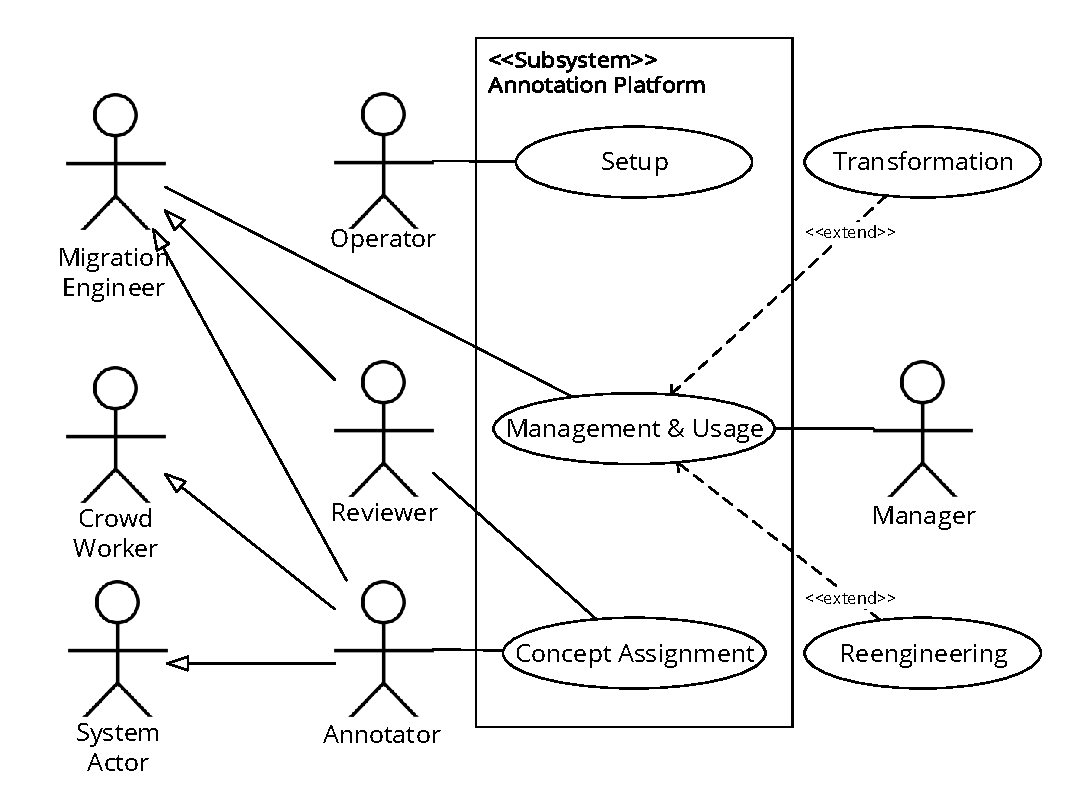
\includegraphics[width=0.85\textwidth]{../figures/awsm-re-use-cases.pdf}
\caption{AWSM:RE Use Cases}\label{fig:awsm.re.use-cases}
}
\end{figure}

The Annotator is the role realizing function \(re\).
This role can be assumed by a human actor i.e.~a \gls{migrationengineer} of the \gls{isv} (cf.~\cref{tbl:stakeholders}), by a system actor, i.e.~a static or dynamic analysis approach as described in \cref{sec:re.related} or by the crowd.
The Annotation Platform is the subsystem of the \gls{awsm} Toolchain that enables the Annotator to create annotations by representing the codebase \(B\) and storing the created annotations in the Knowledge Base \(\mathbb{K}_{B}\).
%The Knowledgebase is a system role equivalent to \(\mathbb{K}_{B}\) which is responsible for storing the annotations created by the Annotator.
The Reviewer is an optional human role required to verify the results of system or crowd Annotators.
Reviewers are \glspl{migrationengineer} of the \gls{isv}.
Manager is a human role that oversees the extraction process (cf.~\cref{tbl:stakeholders}) and manages the \gls{Web Migration} using the information in the Annotation Platform.
The Operator is a human role responsible for the operation of the toolchain and a part of the \gls{isv}'s IT Operations or DevOps staff.

The processes corresponding to the three central use cases are described in the following.
While the Setup Process needs to be performed once, to initiate the environment, the \gls{Concept Assignment} and Management and Usage can be performed multiple times, in parallel and independent of each other.

\vspace{-25pt}
\subsection{Setup Process}
\vspace{10pt}

\begin{figure}[h!]
\hypertarget{fig:awsm.re.setup}{%
\centering
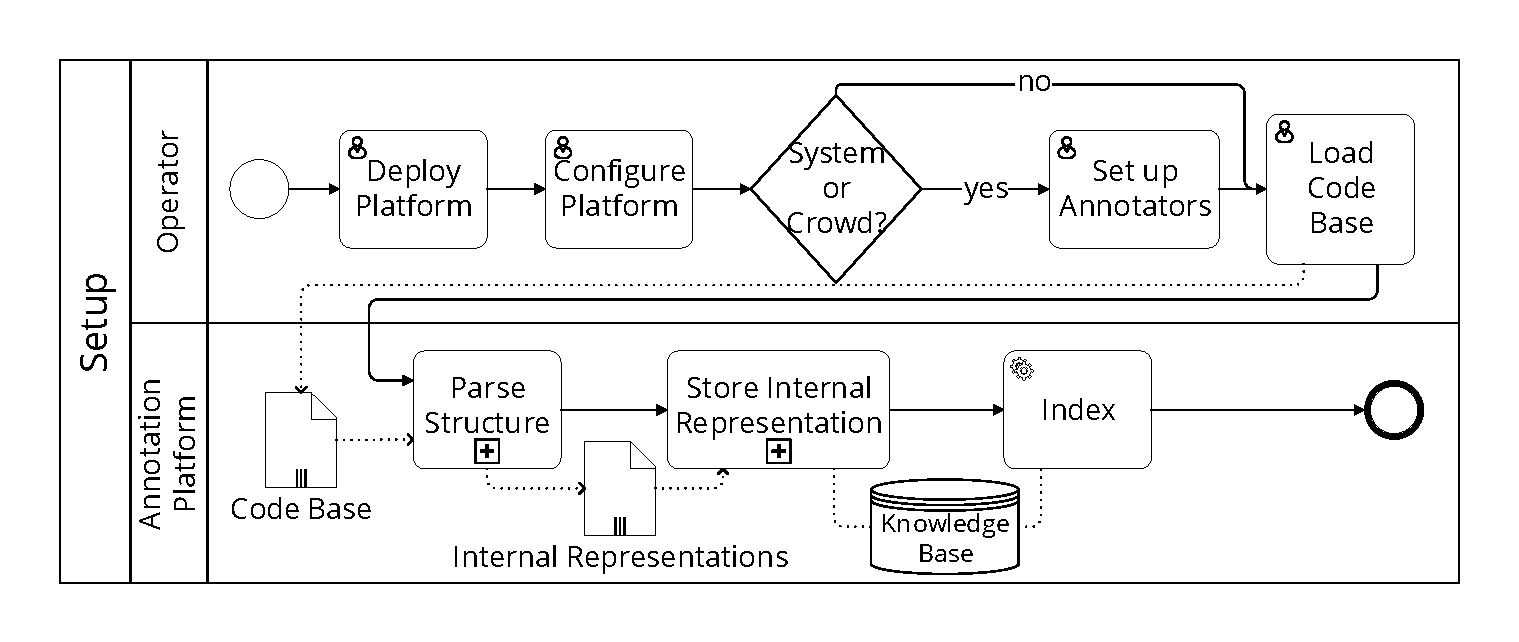
\includegraphics[width=0.99\textwidth]{../figures/awsm-re-setup.pdf}
\caption{Setup Process}\label{fig:awsm.re.setup}
}
\end{figure}

The Setup Process shown in \cref{fig:awsm.re.setup} needs to be executed once, to prepare the Environment for the Knowledge Rediscovery technique.
The Operator sets up the Annotation Platform by deploying it and providing configuration for database connection, authentication, tool integrations etc. 
If realized as system actors, Annotators are set up.
The Operator loads the codebase \(B\) in the Annotation platform, which, by parsing the structure of \(B\), identifies the \gls{Legacy System}'s textual \glspl{artifact} from \(B\) and \(D\) according to the \gls{sckm}, creates internal representations, and performs indexing on the contents.
%Details on the parsing and internal representation are described in \cref{sec:extraction.platform}.

As shown in \cref{fig:awsm.re.concept.assignment}, the Annotator requests an \gls{artifact} \(f\) via the suitable interface of the Annotation Platform, i.e.~the user interface for human actors or the \gls{api} for system actors.
The user interface provides navigation of the information space of textual \glspl{artifact} in \(B\) and \(D\) according to the parsed structure.
It supports filtering based on the internal organization of the code, e.g. for different sofware packages, assemblies etc.
It also supports searching based on full-text indexation of the textual contents.
When selecting an \gls{artifact}, the user interface displays the \gls{artifact} with syntax highlighting and already existing assigned \glspl{Concept} in the Knowledge Base to support the Annotator's understanding of the code.
The Annotator views the \gls{artifact} and performs the \gls{Reverse Engineering} activities of \emph{extraction} and \emph{abstraction} realized as \gls{Concept Assignment}: he identifies a relevant segment \(s \in f\) of the \gls{artifact} and assigns an existing concept (cf.~\cref{def:concept}) to it or creates a new one.
%Integration aspects of the \gls{Concept Assignment} subprocess are described in \cref{sec:re.conceptual.process}.
System actor Annotators interact with the Annotation platform through its \gls{api} and automatically perform extraction and abstraction as defined by the static or dynamic analysis method they implement.
The details of Crowd-based Annotators are described in \cref{sec:csre}.
Optionally, for system actors and Crowd-based Annotators, the Reviewer checks and confirms, declines, or corrects the \glspl{Concept Assignment}.
The annotation process should produce at least one \gls{Concept Assignment} as code annotation \(a\), regardless of the actor.
The Knowledge Base adds the new information to its storage, which consists of a location \(l\) and a knowledge instance \(k\) as defined in the \gls{sckm}.

\vspace{-10pt}
\subsection{Concept Assignment Process}
\vspace{10pt}

\begin{figure}[h!]
\hypertarget{fig:awsm.re.concept.assignment}{%
\centering
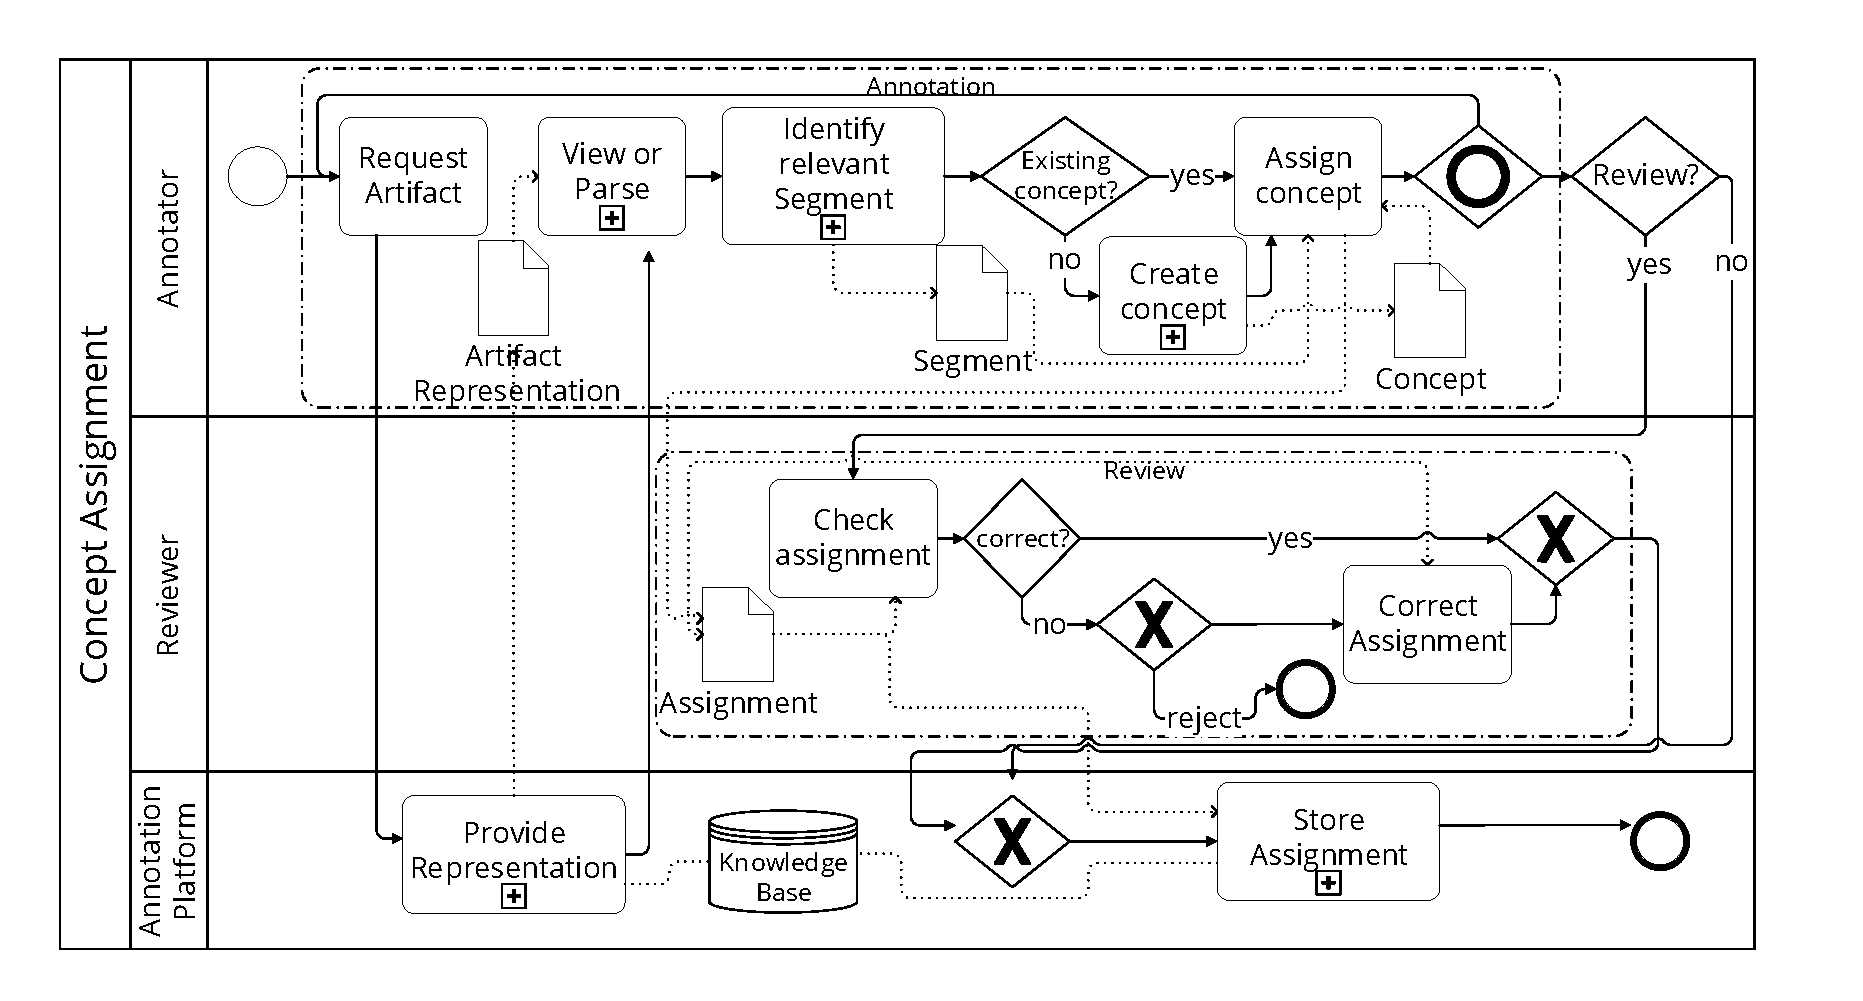
\includegraphics[width=0.99\textwidth]{../figures/awsm-re-concept-assignment.pdf}
\caption{Concept Assignment Process}\label{fig:awsm.re.concept.assignment}
}
\end{figure}

As outlined in requirement \cref{c:4} Agile, integration of \gls{Web Migration} into ongoing development is crucial to reduce additional efforts and address the lack of resources of \glspl{isv}.
The \gls{Concept Assignment} process can be applied in small increments whenever a part of the \gls{Legacy System} needs to be changed for maintenance \autocite{Heil2016AWSM}.
Embedding \gls{Concept Assignment} with ongoing development activities provides several benefits: The effort is lower compared to performing \gls{Concept Assignment} as separate activity because the cognition effort of program comprehension for creating a \emph{mental representation} of the source code \autocite{Pennington1987Mental} in \gls{Forward Engineering} is reused.
Understanding of a specific segment of code gained for maintenance and development is codified during or right after the \gls{Forward Engineering} activity.
Vice versa, availability of knowledge previously extracted can support the comprehension for \gls{Forward Engineering}.
The resulting continuity of \gls{Reverse Engineering} improves the consistency of code and the \knowledgebase.
To support \gls{migrationengineer} stakeholders performing this \gls{Concept Assignment} embedded into ongoing development, integration into editors/\glspl{ide} is required as provided by the Annotation Platform described in \cref{sec:re.impl.integration}.

\vspace{-10pt}
\hypertarget{sec:re.conceptual.process.usage}{%
\subsection{Management and Usage Process}\label{sec:re.conceptual.process.usage}}
\vspace{10pt}

\begin{figure}[h!]
\hypertarget{fig:awsm.re.usage}{%
\centering
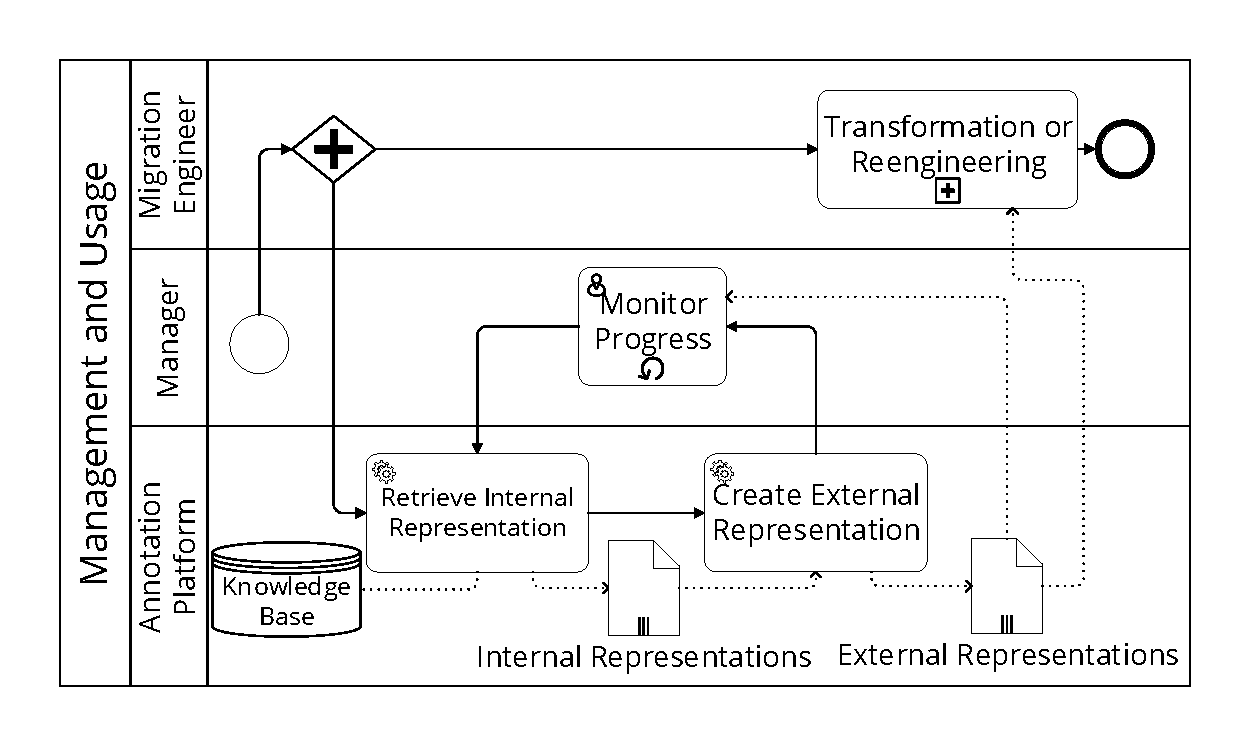
\includegraphics[width=0.99\textwidth]{../figures/awsm-re-usage.pdf}
\caption{Management and Usage Process}\label{fig:awsm.re.usage}
}
\end{figure}
As shown in \cref{fig:awsm.re.usage}, the Platform supports the Manager role to monitor the \gls{Concept Assignment} by providing a suitable external representation -- a user interface with statistics and visualizations of the progress and to understand the as-is business process and rules portfolio of the \glslink{Legacy System}{legacy} application.
It also supports subsequent \gls{Transformation} or \gls{Reengineering} methods at different degrees of human involvement and model-driven adoption (cf.~\cref{p:2} and \cref{p:3}) by representing the Knowledge Base in a human-understandable form via the user interface and an \gls{api} based on open \gls{web} standards (cf.~\cref{p:1}).
This requires a generic, extensible, and queryable knowledge representation model, which is described in \cref{sec:representation}.

Integration with ongoing development activities (requirement \cref{c:4}) of the Management and Usage process is achieved by associating a set of annotations \(A=\{a_1, a_2, \ldots, a_n\}\) with forward development process \glspl{artifact}, i.e.~a set of stories \(S = \{s_1, s_2, \ldots, s_n\}\) in a backlog.
In this way, they form a \emph{migration package} that feeds a \emph{migration backlog} \autocite{Heil2016AWSM} from which stories can be integrated into the planning of iterations, e.g.~into sprint backlogs, achieving integration with agile planning at \glspl{artifact} level.
To support management stakeholders, integration into software project management platforms is required as described as part of the Annotation platform in 
\Cref{sec:re.impl.integration}.

\vspace{-15pt}
\hypertarget{sec:extraction.platform}{%
\section{Annotation Platform}\label{sec:extraction.platform}}
\vspace{15pt}

%``Reverse engineering tools assist the process by working backwards from an existing product to create artifacts such as specification and design descriptions, which can then be transformed to generate a new product from an old one.'' \autocite{SWEBOK2014} 
The \gls{awsmap} \autocite{Heil2016AWSM} \gls{Reverse Engineering} tool contributes to the identification and management of knowledge specified in research objective \cref{ro:1} by supporting the AWSM:RE Knowledge Rediscovery technique and managing the extracted knowledge.
It answer AWSM:RE RQ3 for both system and human users and enables \gls{Concept Assignment} for the three types of Annotators introduced above and implements the \awsmknowledgebase \(\mathbb{K}_{B}\) in \cref{def:kb-formalism}.
\Cref{fig:awsmap} shows its architecture, which was prototypically implemented using C\# .NET 4.5 MVC 5.2.
\begin{figure}[h!]
\hypertarget{fig:awsmap}{%
\centering
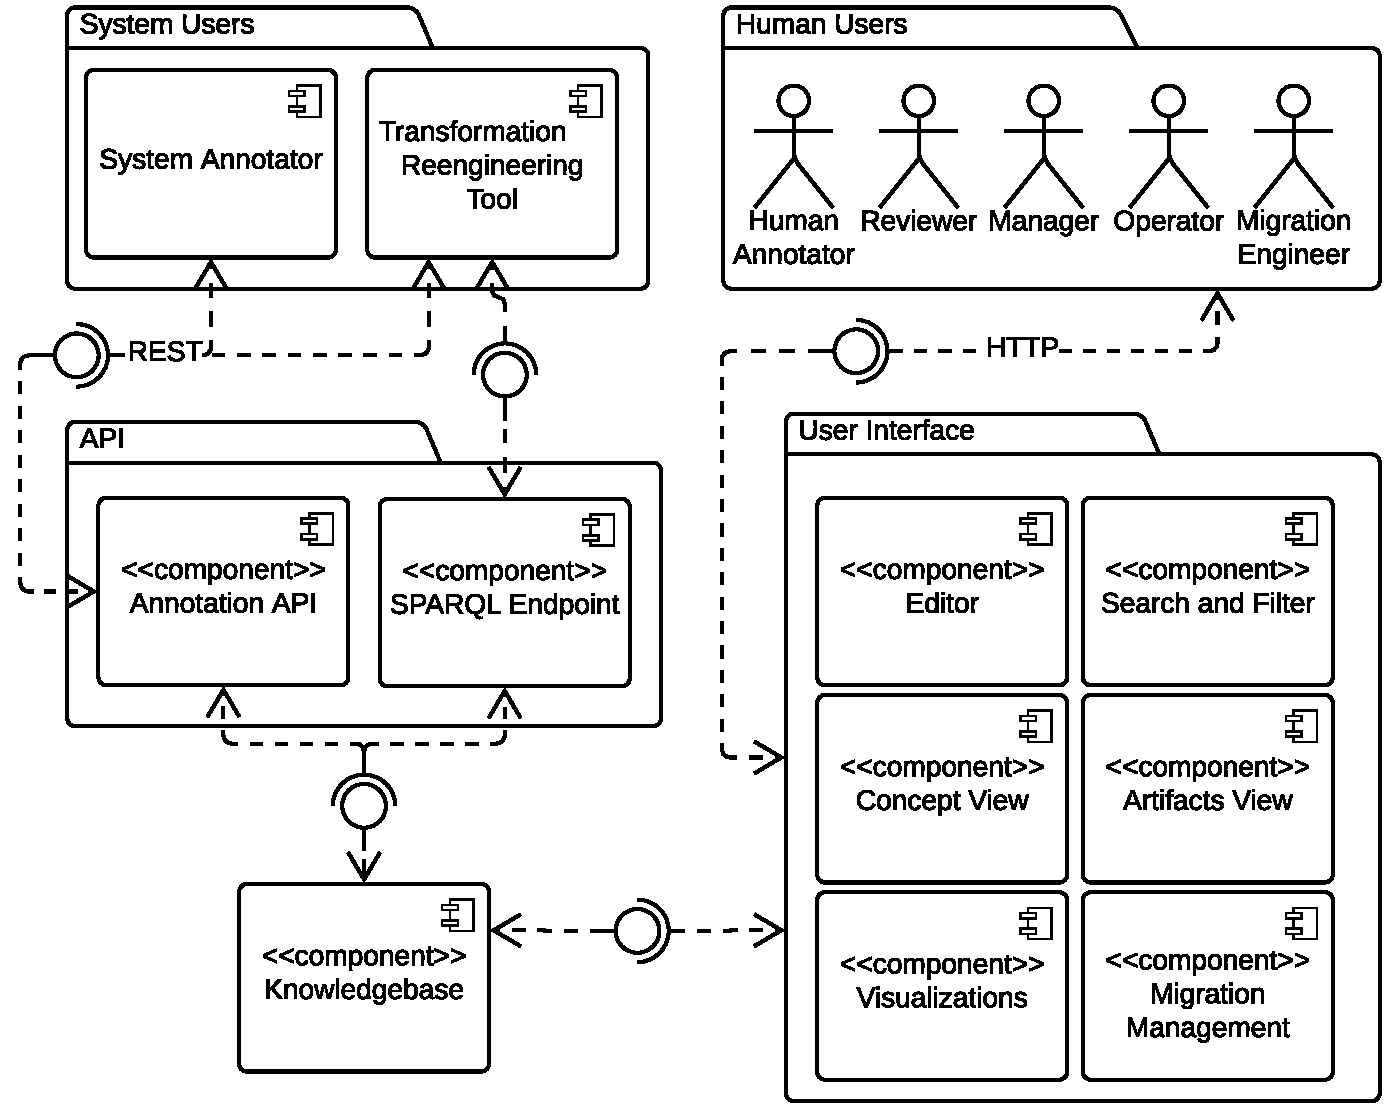
\includegraphics[width=0.9\textwidth]{../figures/awsmap-NOFONTS.pdf}
\caption{AWSMAP Architecture}\label{fig:awsmap}
}
\end{figure}

\gls{awsmap} provides two interfaces over the \awsmknowledgebase: a user interface for supporting human users in the different roles and processes defined in \cref{sec:re.conceptual.process}, and an \gls{api} for supporting system users in annotation and subsequent \gls{Transformation} or \gls{Reengineering}.
The functionality provided to human users via the user interface is described in \cref{sec:re.impl.features}, its integration with the development environment of \glspl{isv} in \cref{sec:re.impl.integration}, and the internal and external knowledge representations for system users via the API is described in \cref{sec:representation}.
%Integration with the existing management and development environment of the \gls{isv} is described in \cref{sec:re.impl.integration}, the queryable external representation layer is described in \cref{sec:re.impl.representation}.

\vspace{-35pt}
\hypertarget{sec:re.impl.features}{%
\subsection{User Functionality}\label{sec:re.impl.features}}
\vspace{10pt}

The \glslink{web}{Web}-based user interface supports \glspl{migrationengineer} to perform \gls{Concept Assignment} and manage domain knowledge, answering AWSM:RE RQ3 for human users.
It displays the structure of the \glslink{Legacy System}{legacy} codebase \(B\), allowing to filter by \gls{kdm} \emph{Module}, i.e.~Visual Studio Solution, and provides a view for each \gls{artifact} \(f \in B\).

\begin{figure}[h!]
\hypertarget{fig:awsmap.editor}{%
\centering
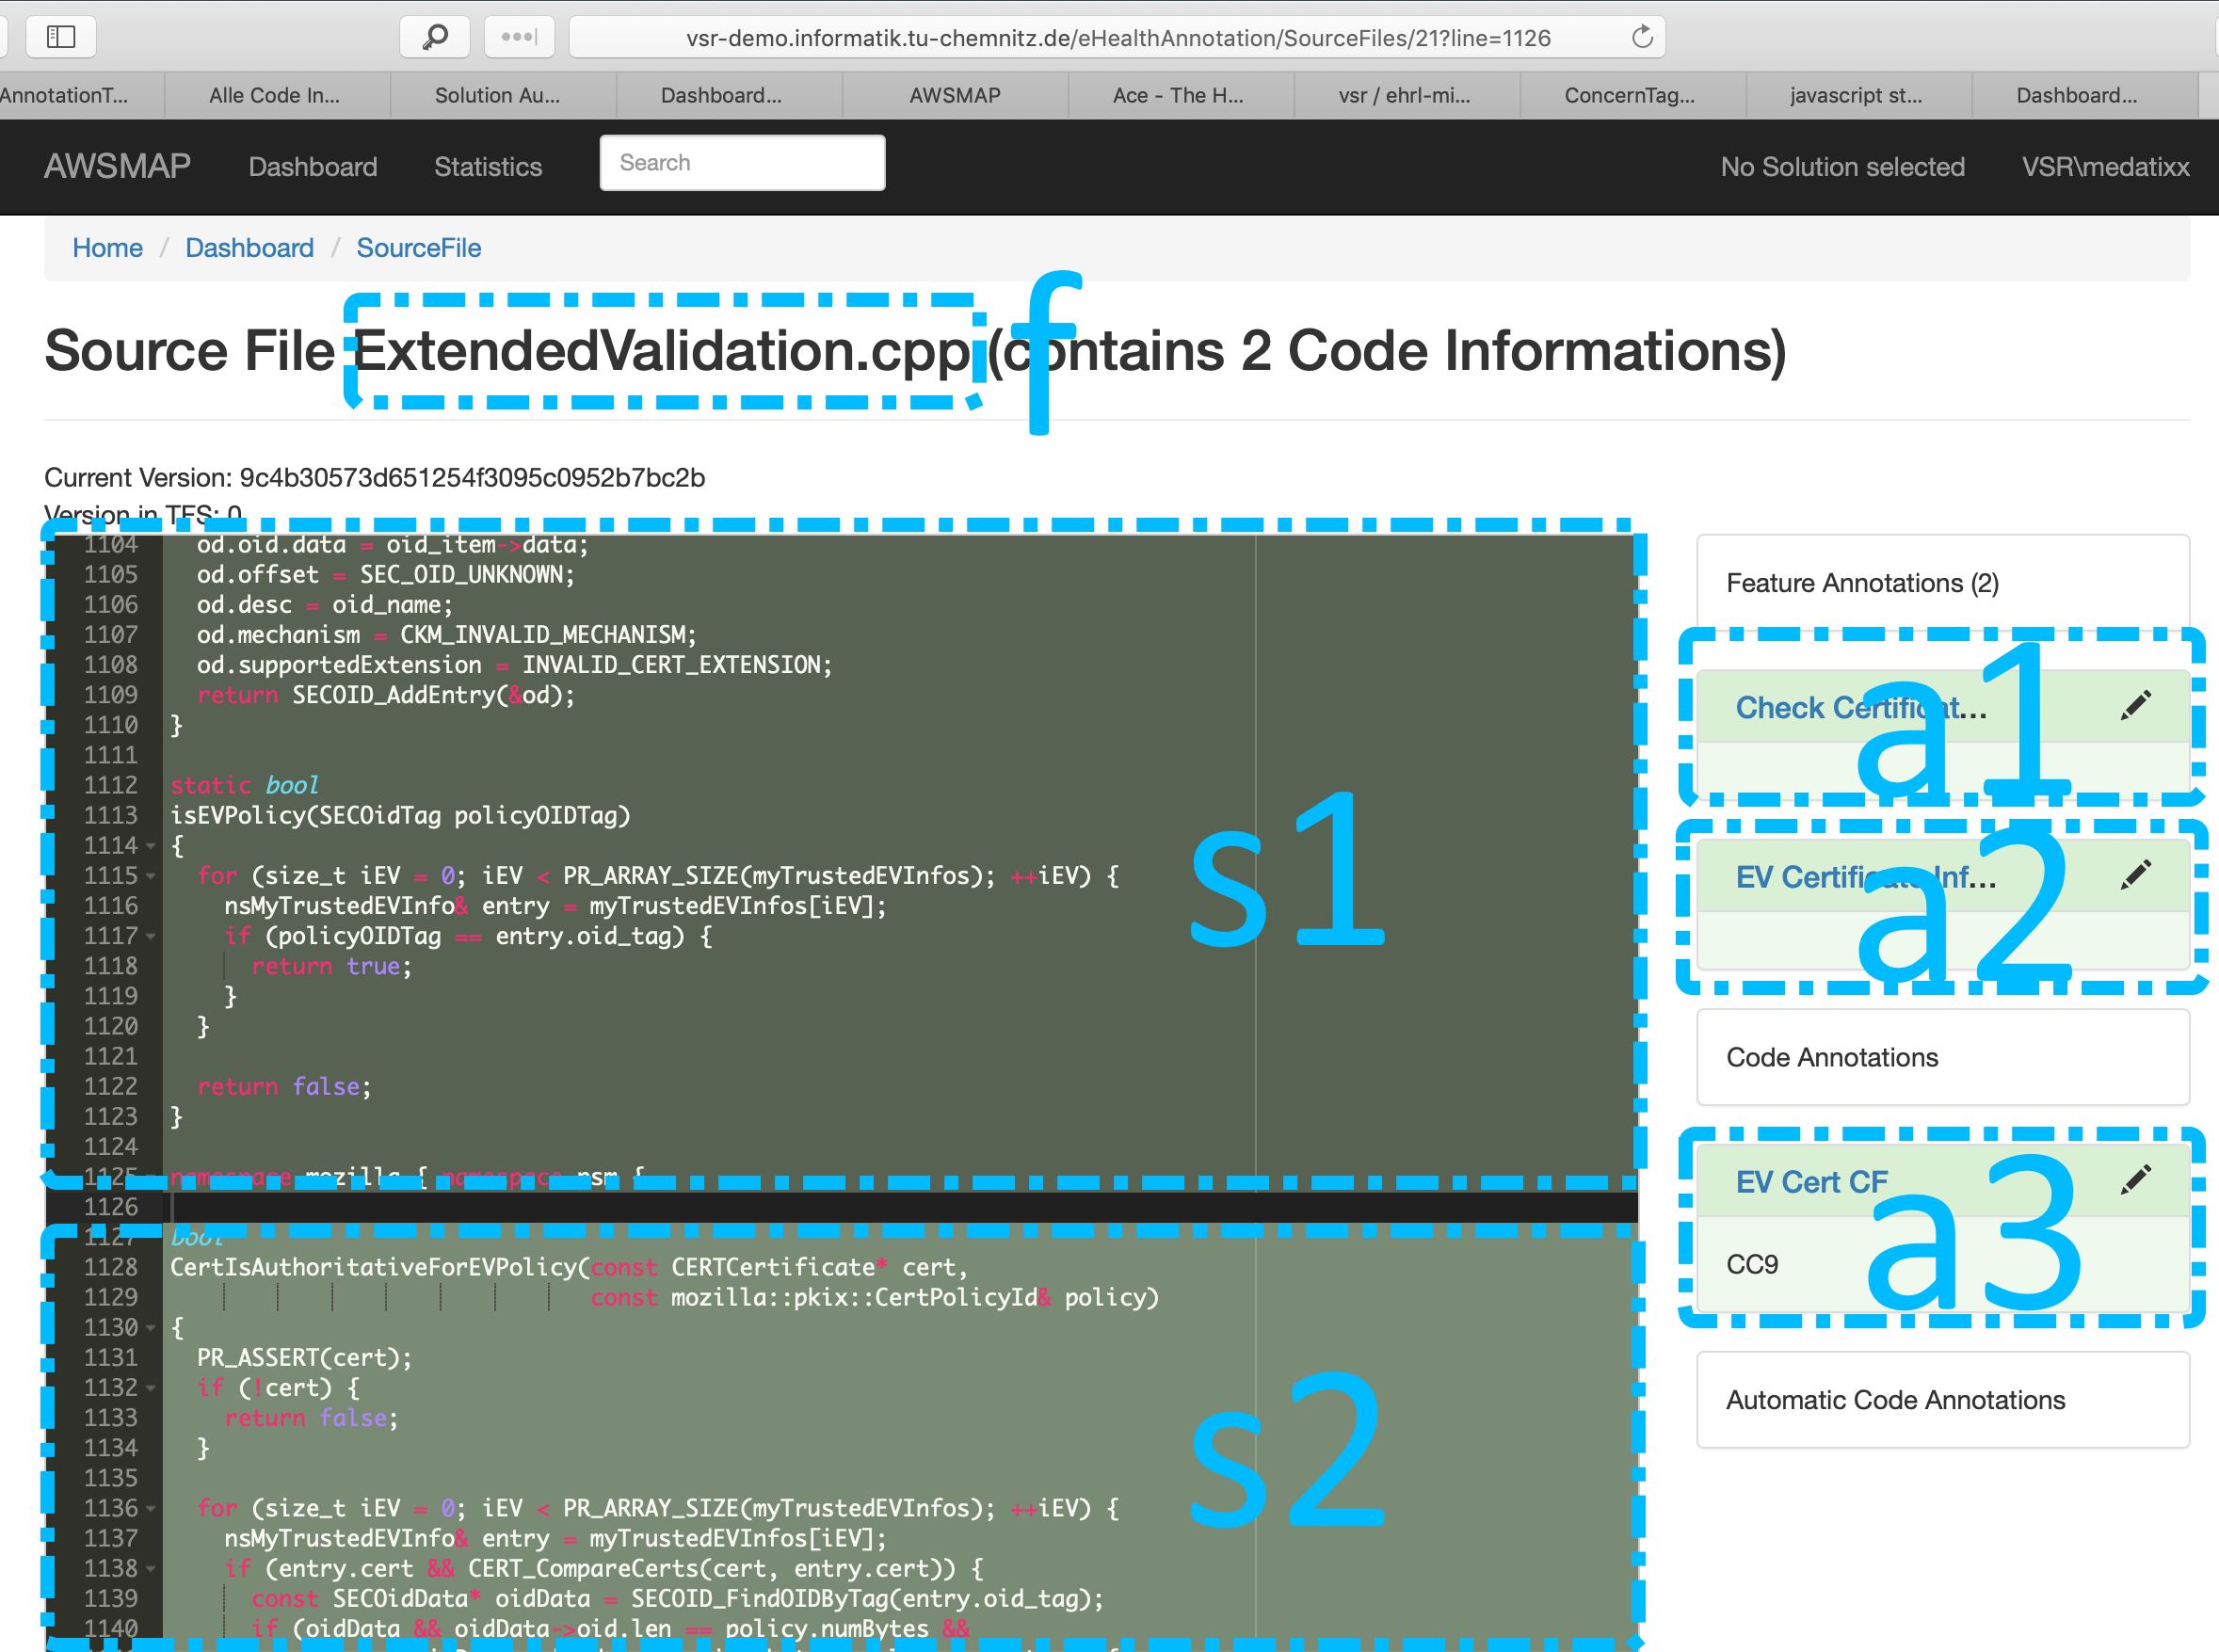
\includegraphics[width=0.85\textwidth]{../figures/screenshots/ap-editor3.png}
\caption{Annotation Platform Editor Screenshot}\label{fig:awsmap.editor}
}
\end{figure}
\vspace{-5pt}

\gls{awsmap} displays artifacts with syntax highlighting ace.js\footnote{\url{https://ace.c9.io/} Retrieved: 6.12.2019}, as shown in \cref{fig:awsmap.editor}.
The content of the artifact \(f\), .e.g the source code, is displayed in the center,
existing annotations \(a_1, a_2, a_3)\) are displayed as overlays and are listed on the right side of the view.
By clicking on an annotation in the list, the content view scrolls to the corresponding location in the artifact.
New annotations can be created by selecting a segment of code \(s\) in the content view, like \(s_1, s_2\) shown in the figure, and selecting an existing or creating a new \gls{Concept}.
The representation of the assigned \gls{Concept} can be viewed by following the link in the annotation.
The Concept View that is opened is shown in \cref{fig:awsmap.concept}.
\begin{figure}[h!]
\hypertarget{fig:awsmap.concept}{%
\centering
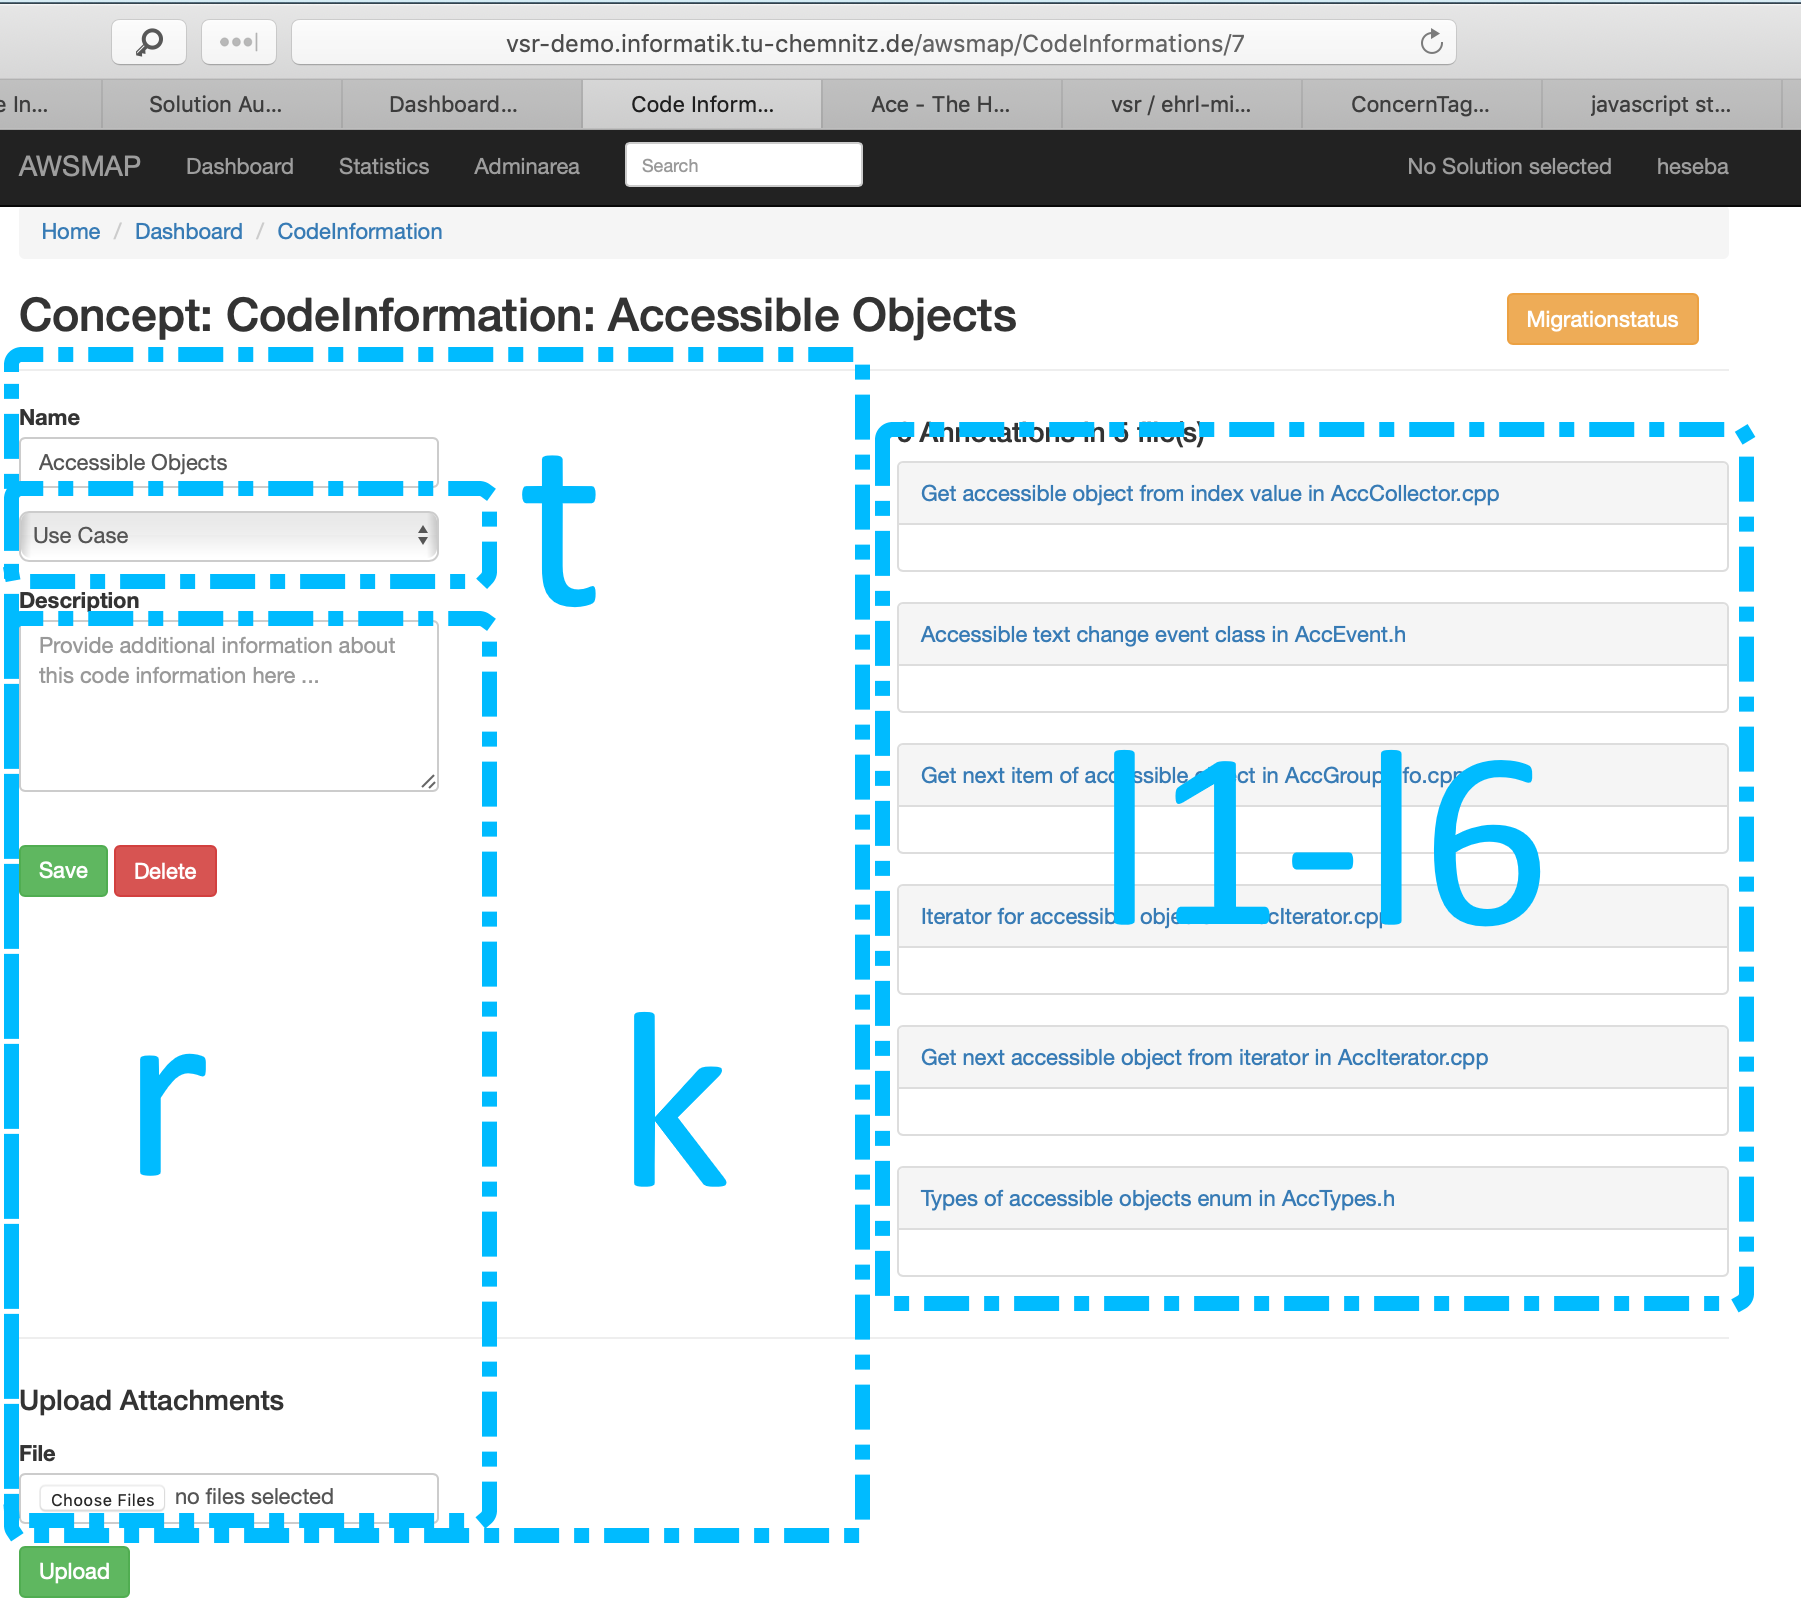
\includegraphics[width=0.85\textwidth]{../figures/screenshots/ap-concept3.png}
\caption{Annotation Platform Concept View}\label{fig:awsmap.concept}
}
\end{figure}
It shows a knowledge instance \(k=(t,r)\), displaying the \gls{Concept}'s name, type \(t\), and description.
Additionally, attachments can be uploaded, e.g.~\gls{uml} or \gls{bpmn} diagrams or other \glspl{artifact} specific for subsequent processing (cf.~\cref{p:2} and \cref{p:3}).
Locations \(l_1\)-\(l_6\) of the \gls{Concept} in \(B\) are listed on the right side with the links leading to the corresponding segment \(s\) in \gls{artifact} \(f\).
%
%ConcernTagger \autocite{Eaddy2008aConcernTagger} is a conceptually similar tool, but it does not provide a \glslink{web}{Web}-based user interface and is a separate tool in contrast to the integrated \gls{awsmap} platform.
%
One of the core benefits of \gls{awsmap} is referencability of all \glspl{artifact} and knowledge through individual URLs, as seen in the address bar in \cref{fig:awsmap.concept}.
This implements hypertext-based navigation of the \glslink{Legacy System}{legacy} information hyperspace and fosters integration by making knowledge linkable in internal email or chat communications, intranet wikis, blogs, etc.
%\vspace{-5pt}

For Management stakeholders, \gls{awsmap} provides a UI with different monitoring statistics and visualizations of \gls{Concept} structure.
\Cref{fig:awsmap.statistics} shows Annotator statistics, providing an overview of the annotation progress and individual Annotator performance.
\pagebreak 
\begin{figure}[h!]
\hypertarget{fig:awsmap.statistics}{%
\centering
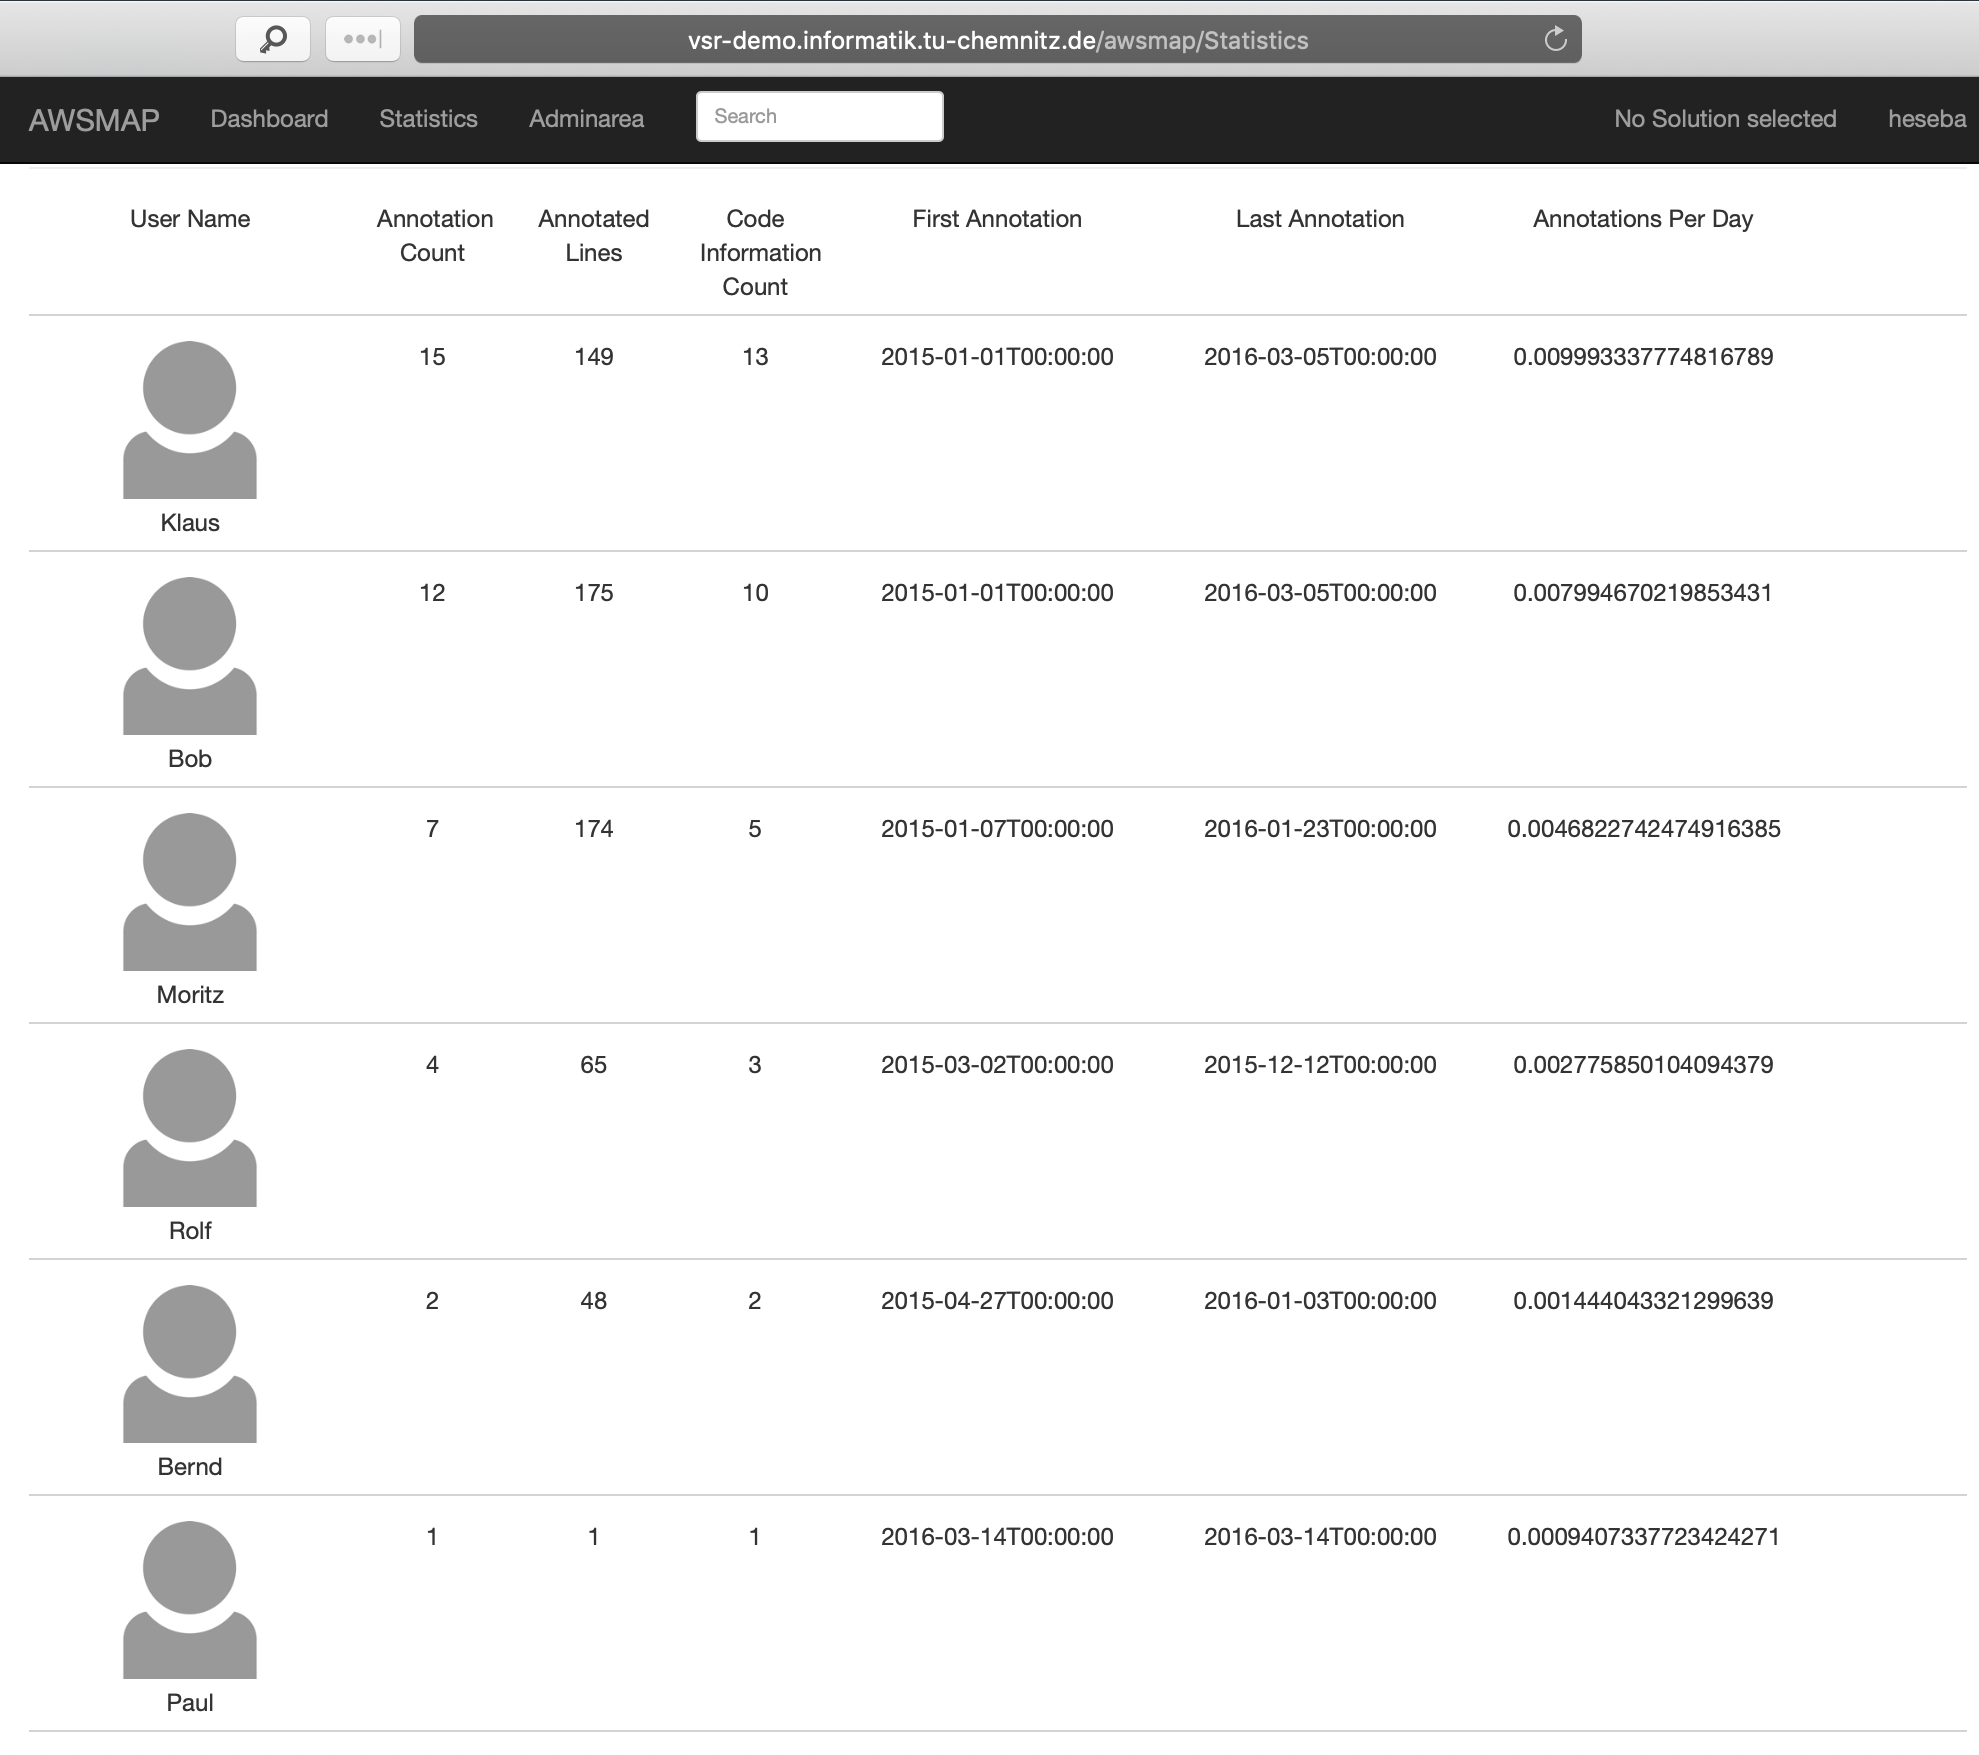
\includegraphics[width=0.78\textwidth]{../figures/screenshots/ap-statistics-result2.png}
\caption{Annotation Platform Statistics}\label{fig:awsmap.statistics}
}
\end{figure}

Based on the existing annotations, \gls{awsmap} provides software quality visualizations allowing to assess structural problems of the legacy code that need special consideration before or during \gls{Web Migration}.
The focus of the visualizations is on interlacing between \glspl{artifact}, features, and knowledge instances in different combinations.
\Cref{fig:awsmap.sankey} shows a Sankey Diagram of \gls{artifact}-feature interlacing.
\glspl{artifact} \(f\) are displayed on the left side, features \(k=(t,r)\) with \(t \in {\mathrm{user story}, \mathrm{use case}, \ldots}\) on the right side.
The connections between them represent occurrence of features in the artifacts, the width of the connection increases with the number of corresponding annotations.
The more chaotic, i.e. the more entangled the connecting lines are, the higher the interlacing, indicating a lack of separation of concerns.
Individual connections can be highlighted, and the \gls{artifact} and feature names are links leading to the corresponding location in the source code for further inspection.
Other visualizations implemented in \gls{awsmap} are Force Graphs and Chord diagrams.
\begin{figure}[h!]
\hypertarget{fig:awsmap.sankey}{%
\centering
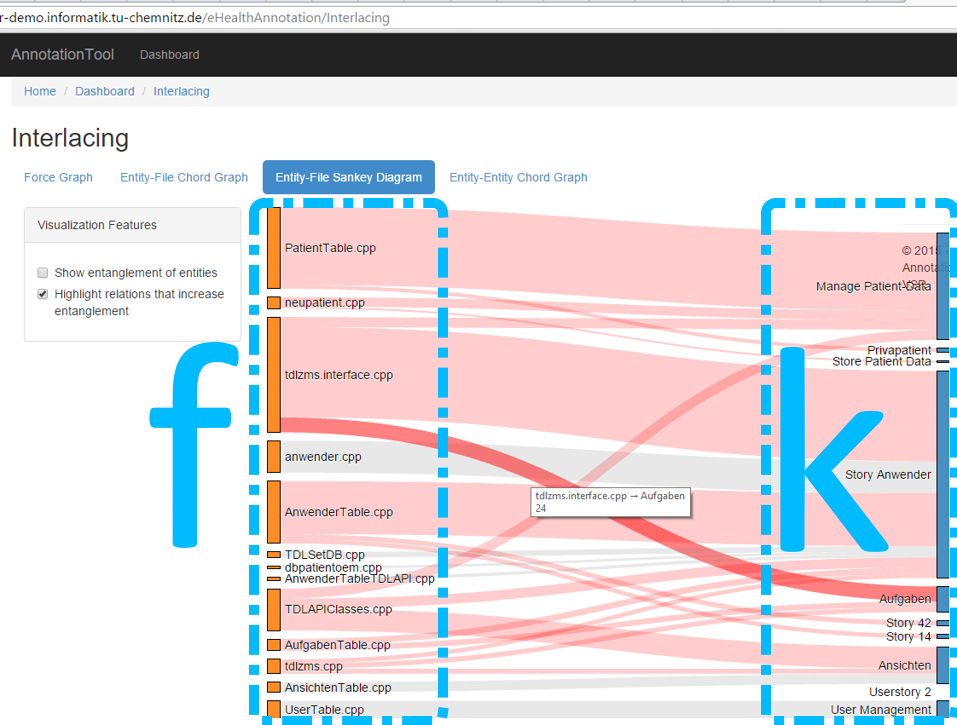
\includegraphics[width=0.78\textwidth]{../figures/screenshots/sankey2.png}
\caption{Annotation Platform Visualizations}\label{fig:awsmap.sankey}
}
\end{figure}

\vspace{-10pt}
\hypertarget{sec:re.impl.integration}{%
\subsection{Integration in ISV environments}\label{sec:re.impl.integration}}
\vspace{10pt}

This section addresses integration of \gls{awsmap} into core parts of the environment of \glspl{isv}: Integrated Development Environments, Version Control Systems, Project Management Platforms, and Authentication and Authorization Systems.
\Cref{fig:awsmap.integration} provides an overview of the integration architecture of \gls{awsmap}.
The following paragraphs provide one example for each of these integrations, which was prototypically implemented in \gls{awsmap} for the specific environment of the scenario stakeholder, as described in \cref{sec:scenario}.
\begin{figure}[h!]
\hypertarget{fig:awsmap.integration}{%
\centering
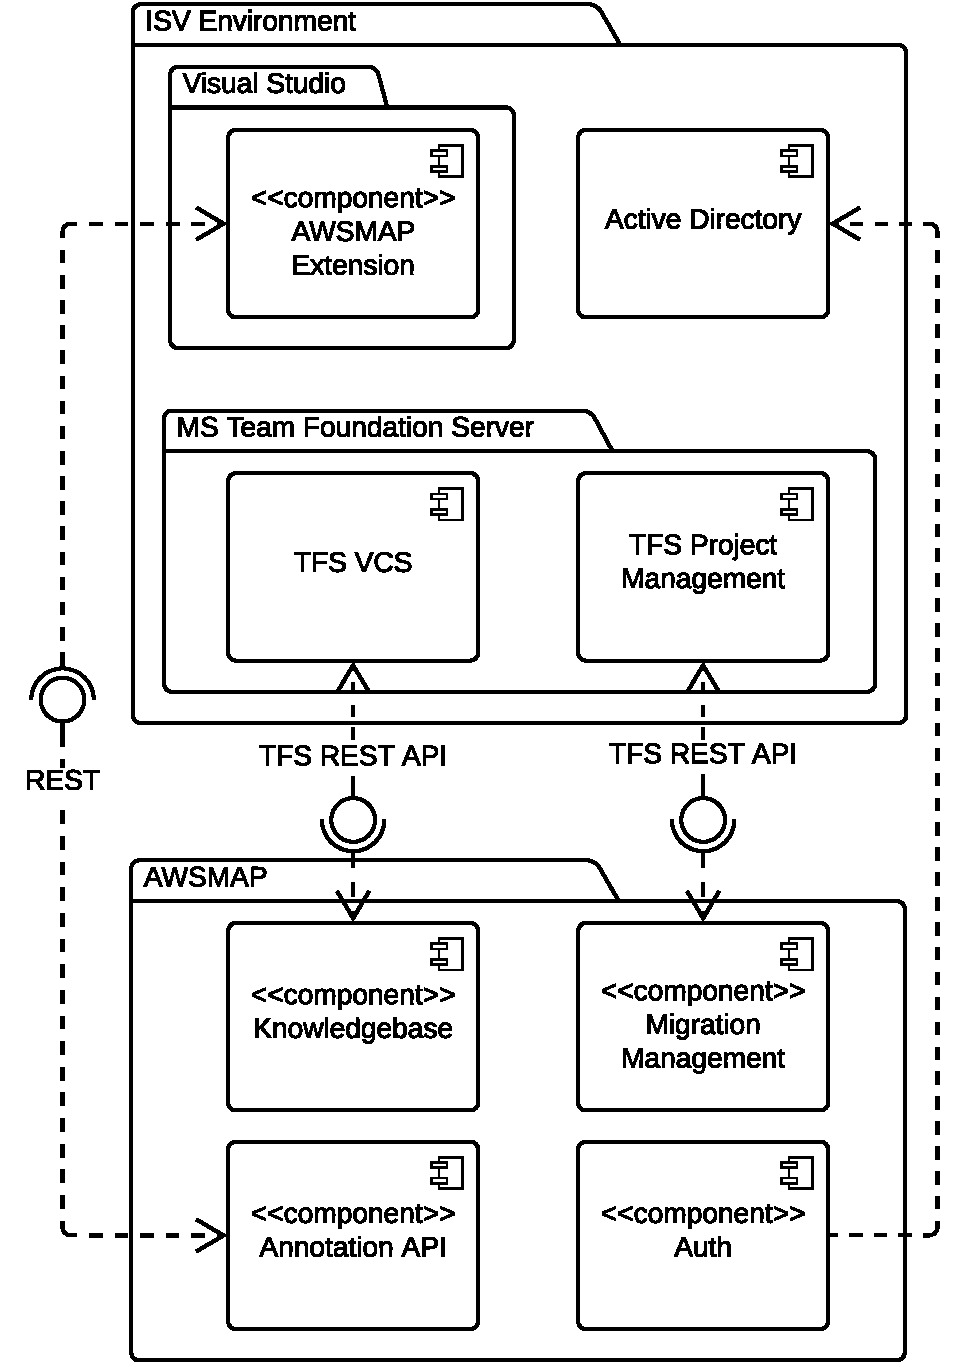
\includegraphics[width=0.75\textwidth]{../figures/awsmap-integration-NOFONTS.pdf}
\caption{AWSMAP Integration Architecture}\label{fig:awsmap.integration}
}
\end{figure}

\textbf{Integrated Development Environment Integration.} Software engineers of \glspl{isv} create and manage \glspl{artifact} of a software system using an environment of development tools.
Typically \emph{Integrated Development Environments (\glspl{ide})} are used for these activities.
%Reverse engineering tools should be integrated into development environments to facilitate adoption by \glspl{migrationengineer} instead of being built as separate tools \autocite{Muller2000}.
\gls{awsmap} supports integration into \glspl{ide} via its \glslink{rest}{RESTful} \gls{api} in order to facilitate the integration of AWSM:RE Knowledge Rediscovery into ongoing development as specified in \cref{sec:re.conceptual.process}.
The implementation in the context of \cref{sec:scenario} is realized as Visual Studio Extension, presented in \cref{fig:awsmap.ide}.
\begin{figure}[h!]
\hypertarget{fig:awsmap.ide}{%
\centering
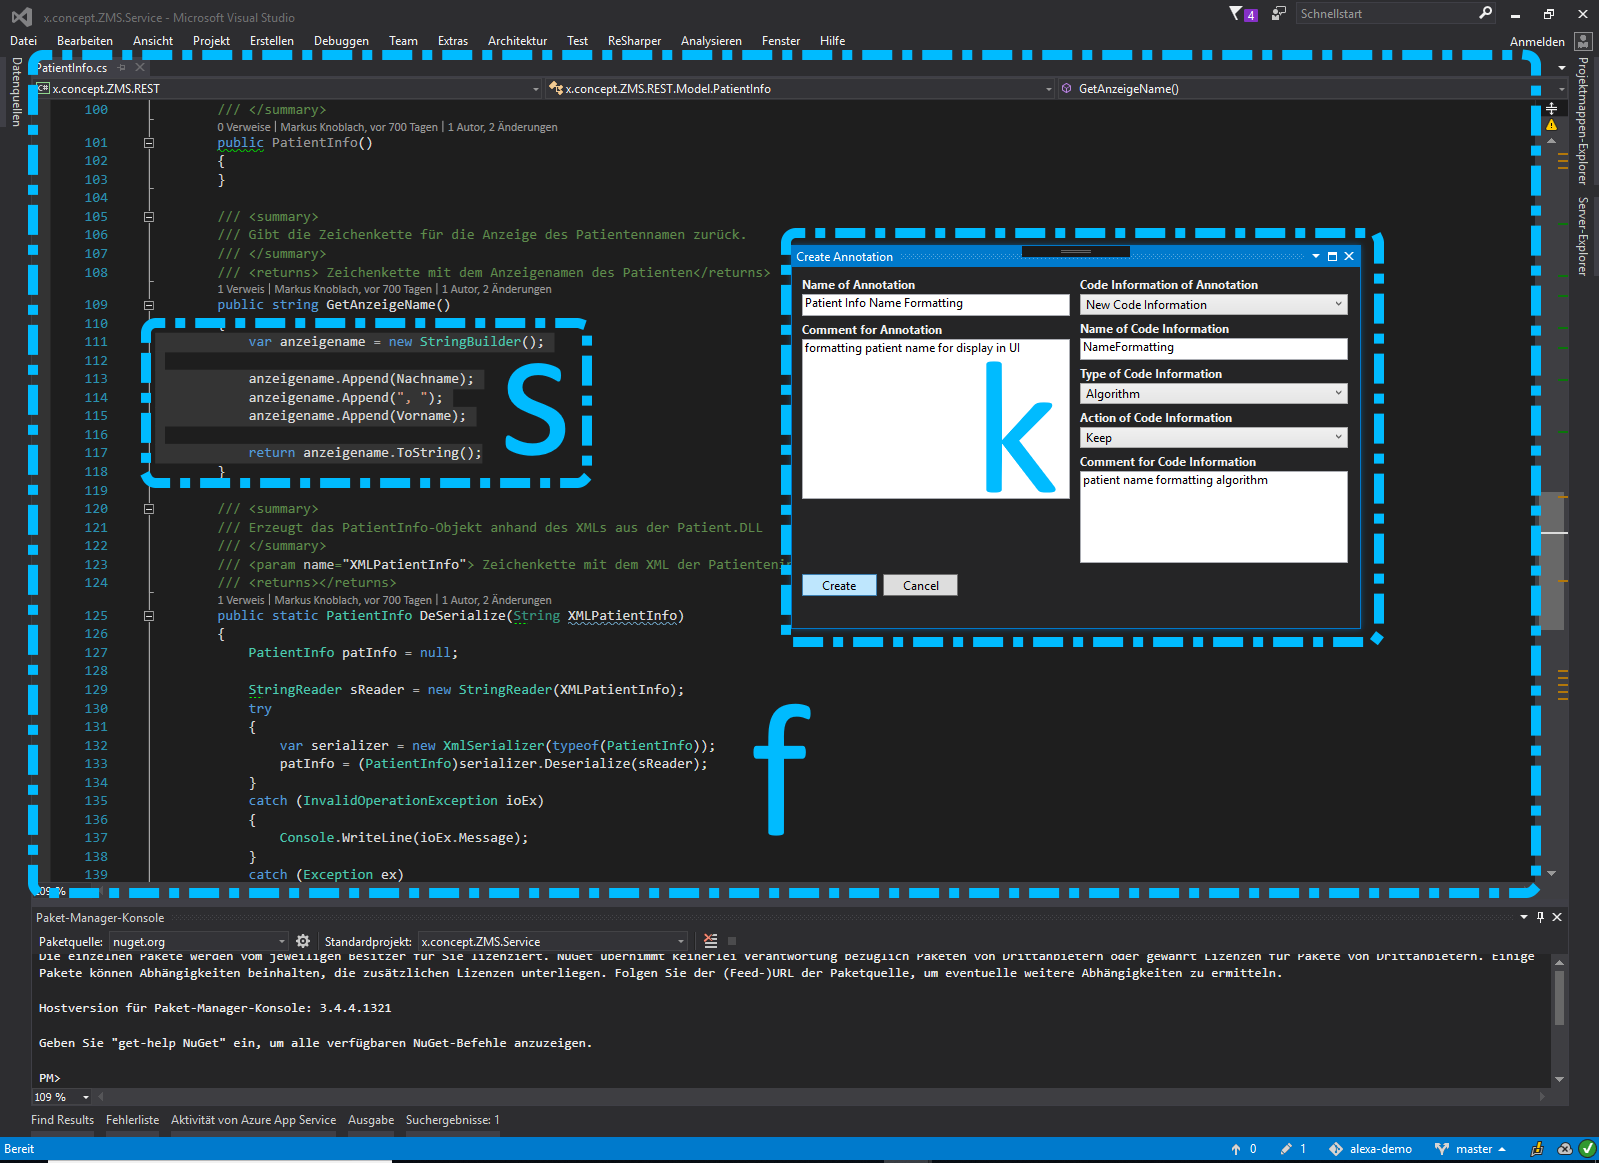
\includegraphics[width=0.99\textwidth]{../figures/screenshots/ide-integration-hd2.png}
\caption{AWSMAP IDE Integration}\label{fig:awsmap.ide}
}
\end{figure}
The screenshot shows creation of a new annotation on an \gls{artifact} \(f\), highlighting a segment \(s\) and entering information about knowledge instance \(k\).
Paper prototypes and interactive MS PowerPoint-based wireframes were used for collaborative design (cf.~Co-Creation \autocite{HCD2015}) of the \gls{ide} integration with \gls{isv} Software Engineers.
\Cref{fig:awsmap.ide} shows the creation of a new annotation in the Visual Studio Extension.
A part of the source code can be selected in the IDE's source code editor, by right-clicking and selecting ``Create Annotation'' in the menu, the dialog displayed on the right side opens.
It captures the same data as the corresponding view in the \gls{web} user interface of \gls{awsmap} and synchronizes annotations via the \glslink{rest}{RESTful} \gls{api}.
%\todo{Only recently, similar approaches like codestream slack integration}
%https://www.golem.de/news/programmierung-codestream-ermoeglicht-diskussionen-am-code-per-slack-1908-142998.html

\textbf{Version Control Integration.} For typical \glspl{isv}, the \glspl{artifact} of the \gls{Legacy System} \(\mathfrak{L}\) are under version control using a \emph{\gls{vcs}}.
\gls{awsmap} supports \gls{vcs}-integration by implementing the ``load codebase'' step in \cref{fig:awsm.re.setup} as import from an existing \gls{vcs} repository.
In the context of \cref{sec:scenario}, \gls{vcs} integration was implemented using the \gls{tfs} \gls{rest} \gls{api}\footnote{\url{https://docs.microsoft.com/en-us/rest/api/azure/devops/?view=azure-devops-rest-5.0} Retrieved: 6.12.2019}.
The Operator specifies the \gls{tfs} instance configuration and repository URL in the \gls{awsmap} web.config in the ``configure toolchain'' step of \cref{fig:awsm.re.setup} and can then trigger import and parsing of the codebase from \gls{tfs} \gls{vcs} via the Admin Dashboard.

\textbf{Project Management Integration.} For Management stakeholders, \gls{awsmap} integrates with \gls{tfs} \emph{project management} capabilities via the \gls{tfs} \gls{rest} \gls{api}.
Integration with ongoing agile development is achieved in the context of the \gls{tfs} Scrum Process Template.
The migration packages described in \cref{sec:re.conceptual.process.usage} are represented as work items of type feature, its contents as backlog items with parent relationships to the migration package.
URLs pointing to the corresponding entity in \gls{awsmap} are added to the descriptions, and URLs to the entity in the \gls{tfs} \gls{web} \gls{ui} are added to \gls{awsmap} entities to allow switch between the two contexts.
\Cref{fig:tfs-integration} shows a screenshot of the definition of a migration package in \gls{awsmap}.
\begin{figure}[h!]
\hypertarget{fig:tfs-integration}{%
\centering
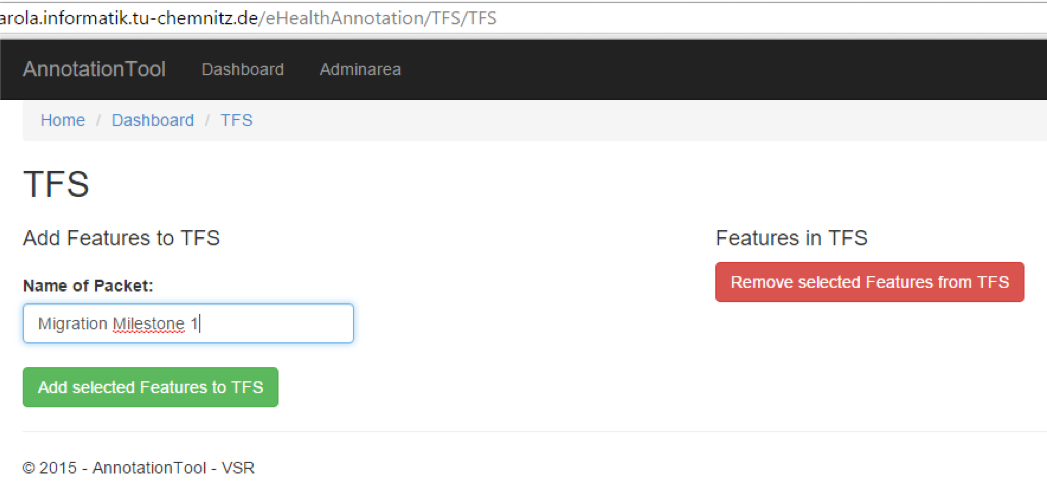
\includegraphics[width=0.85\textwidth]{../figures/screenshots/tfs-integration-migrationpackages.png}
\caption{TFS Integration: Migration Packages}\label{fig:tfs-integration}
}
\end{figure}

\textbf{Authentication and Authorization Integration.} The last integration aspect is \emph{authentication and authorization} of users.
\glspl{isv} typically operate an Identity Provider to restrict access to their company-internal resources.
In the context of \cref{sec:scenario}, \emph{Active Directory (AD)}\footnote{\url{https://docs.microsoft.com/de-de/windows-server/identity/active-directory-federation-services} is used, thus \gls{awsmap} Retrieved: 6.12.2019} integrates with AD for federated authentication, allowing users to login with their domain accounts.

\vspace{-10pt}
\hypertarget{sec:representation}{%
\subsection[Queryable Legacy Knowledge Base Repres.]{Queryable Legacy Knowledge Base Representation}\label{sec:representation}}
\vspace{10pt}

This section addresses the system actor perspective of AWSM:RE RQ3, the management of extracted problem and solution domain knowledge, and the provision of this knowledge for further usage in \gls{Web Migration} processes based on \gls{Reengineering} or \gls{Transformation} at different degrees of model-driven adoption.
The challenge is to provide an external representation of the \awsmknowledgebase, as specified in \cref{fig:awsm.re.usage}, which is suitable for various different \gls{Web Migration} approaches.
Thus, the next two subsections describe the representation of knowledge in the \awsmknowledgebase as ontology and the support for querying.

\vspace{-10pt}
\subsubsection*{SCKM Ontology}
\glspl{migrationengineer} require knowledge representations depending on the specific \gls{Transformation} or \gls{Reengineering} process.
The variety of knowledge and models is high, since AWSM:RE addresses knowledge at \gls{psm} or \gls{cim} level of abstraction as resulting from design recovery and is designed for integration with existing \gls{Web Migration} approaches at different degrees of model-driven adoption (principles \cref{p:2} and \cref{p:3}).
This requires a generic and extensible model allowing to associate arbitrary knowledge models with \glslink{Legacy System}{legacy} codebases.

Thus, AWSM:RE implements the \gls{sckm} as \emph{Ontology of knowledge in \glspl{Legacy System}} using the \emph{Web Ontology Language (\gls{owl})}\footnote{\url{https://www.w3.org/TR/owl-overview/} Retrieved: 6.12.2019} \autocite{Heil2016AWSM}.
This allows for a generic knowledge representation that can be extended and integrated with knowledge from external \gls{lod} sources, semantics, and reasoning, using SPARQL\footnote{\url{https://www.w3.org/TR/sparql11-overview/} Retrieved: 6.12.2019} as powerful and model-independent query language and enables access to the rich open \gls{web} standards-based environment and existing infrastructure in the context of the \emph{Semantic Web}.
The SCKM Ontology was designed based on the \gls{sckm} using Protégé\footnote{\url{https://protege.stanford.edu/} Retrieved: 6.12.2019}.
\Cref{fig:ontology} shows the main \gls{owl} classes of the ontology.

\begin{figure}[h!]
\hypertarget{fig:ontology}{%
\centering
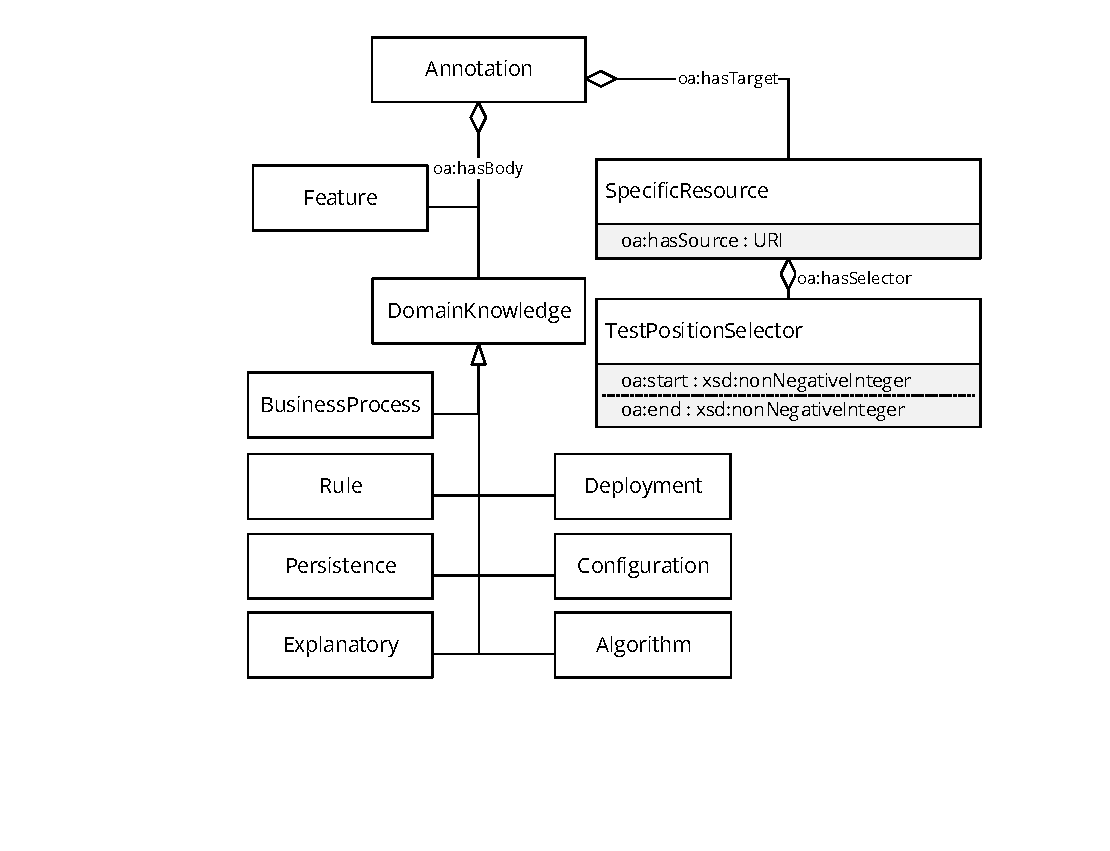
\includegraphics[width=0.75\textwidth]{../figures/awsm-re-ontology.pdf}
\caption{OWL SCKM Ontology Classes}\label{fig:ontology}
}
\end{figure}
The root \texttt{Annotation} class is equivalent to an \gls{sckm} annotation as defined in \cref{def:annotation}.
It is modeled using the \gls{w3c} \gls{oa} \autocite{W3C2017OA}, to allow for portability and sharing across tools.
An \gls{sckm} annotation \(a=(k, l)\) is modeled as \gls{w3c} \gls{oa} annotation with the object properties \texttt{oa:hasBody} pointing to the knowledge payload \(k\) and \texttt{oa:hasTarget} to location \(l\).
Valid bodies are \texttt{Feature} and \texttt{DomainKnowledge} \autocite{Heil2016AWSM}, which can be of any of the \gls{sckm} problem and solution domain types defined in \cref{sec:formalisms.sckm}.
To model the target \(l = (s,f)\), an \texttt{oa:SpecificResource} is used, that references the \glslink{Legacy System}{legacy} \gls{artifact} \(f\) (a \gls{kdm} SourceFile) as URI via \texttt{oa:hasSource}.
Segment \(s=(\alpha, \omega)\) (a \gls{kdm} SourceRegion) is represented as \texttt{oa:TextPositionSelector} via the \texttt{oa:hasSelector} property.
The start \(\alpha\) and end \(\omega\) of the segment are 0-based index numbers in the character stream of \(f\) represented as \texttt{oa:start} and \texttt{oa:end}.
The complete SCKM Ontology can be seen in \cref{sec:sckm-ontology}.

\subsubsection*{Querying Support}
To allow filtering the information in the potentially large \awsmknowledgebase according to information requirements of the \gls{Transformation} or \gls{Reengineering} approaches in use, a key factor is the ability to query the \knowledgebase.
While there is a variety of querying languages for model-driven approaches, e.g. \gls{qvt} introduced in \cref{sec:adm}, these are specific for particular model-driven \gls{Web Migration} approaches and technologies.
Following the design decision of \cref{p:1}, the representation and the query language should instead be based on open \gls{web} standards.
Therefore, the \awsmknowledgebase \(\mathbb{K}_{B}\) can be queried using the SPARQL Endpoint shown in \cref{fig:awsmap} to retrieve a set of \gls{rdf}\footnote{\url{https://www.w3.org/RDF/} Retrieved: 6.12.2019} triples according to the ontology introduced above, serialized in one of the \gls{rdf} notations (e.g.~N3, Turtle, \gls{xml}, etc.) available.
This allows for interoperability based on open \gls{web} standards and supports querying via SPARQL.
To support complex use cases, the \gls{awsmap} SPARQL Endpoint supports reasoning.
This can be demonstrated with the following example.

When querying Knowledge Bases representing knowledge instances in legacy codebases, queries can become unnecessarily complex due to encoding location-related semantics in the query.
Querying all knowledge within a certain area \(s_a\) in an \gls{artifact} \(f\), the semantics of containment need to be expressed in \texttt{FILTER} statements like:

\begin{lstlisting}[language=sparql, captionpos=t, caption=Partial SPARQL Containment Query]
FILTER(
	( ?end > ?astart && ?end <= ?aend ) 
	|| 
	( ?start >= ?astart && ?start < ?aend )
).
\end{lstlisting}

\vspace{-15pt}
This definition of 1-dimensional containment is part of the domain modeled by the \gls{owl} ontology and should not need to be encoded, neither in queries nor explicitly in the data.
Similar to GeoSPARQL\footnote{\url{http://www.geosparql.org/} Retrieved: 6.12.2019}, a query should simply state:

\begin{lstlisting}[language=sparql, captionpos=t, caption={[Partial SPARQL Containment Query using sckm:within]Partial SPARQL Containment Query using sckm:within Property}]
?annotation sckm:within ?area
\end{lstlisting}

Likewise, complex relationships like knowledge-influences-feature should be interfaced as simple triple patterns.
The \gls{awsmap} Querying Support realizes this, by extending the Ontology with additional rules using the \emph{Semantic Web Rule Language (SWRL)\footnote{\url{https://www.w3.org/Submission/SWRL/} Retrieved: 6.12.2019}}.
SWRL allows defining inference rules based on which additional triples are asserted into the knowledge graph.
The following shows an example of a SWRL rule in the Ontology defining the \texttt{influences}-relationship.
The complete list of SWRL rules for Querying Support can be seen in \cref{sec:sckm-ontology-rules}.

\begin{lstlisting}[language=sparql, captionpos=t, caption=SWRL Rules for sckm:influences, label=lst:swrl]
oa:Annotation(?AF) ^ oa:Annotation(?AR) ^ sckm:Feature(?F) ^ sckm:Knowledge(?R) ^ oa:body(?AF, ?F) ^ oa:body(?AR, ?R) ^ oa:SpecificResource(?SR) ^ oa:SpecificResource(?SF) ^ oa:target(?AF, ?SF) ^ oa:target(?AR, ?SR) ^ oa:source(?SF, ? S) ^ oa:source(?SR, ?S) ^ oa:TextPositionSelector(?TR) ^ oa:TextPositionSelector(?TF) ^ oa:selector(?SF, ?TF) ^ oa:selector(?SR, ?TR) ^ oa:start(?TR, ?sr) ^ oa:start(?TF, ?sf) ^ oa:end(?TR, ?er) ^ oa:end(?TF, ?ef) ^ swrlb:greaterThanOrEqual(?er, ?sf) ^ swrlb:lessThan(?sr, ?sf) ^ swrlb:greaterT- hanOrEqual(?ef, ?er) => sckm:influences(?R, ?F)
\end{lstlisting}

\vspace{-10pt}
\hypertarget{sec:csre}{%
\section{Crowdsourced Reverse Engineering}\label{sec:csre}}
\vspace{10pt}

To answer AWSM:RE RQ2 in \cref{sec:re.research-questions}, this section specifies the \gls{Concept Assignment} process in \cref{fig:awsm.re.concept.assignment} for Crowd Annotators \autocite{Heil2018CSRE,Heil2019CSRECCIS}.
As outlined in \cref{sec:re.conceptual.process}, the Annotator role can be impersonated by \gls{isv} staff, an automated system, or the crowd.
To address the limited resources constraint in \cref{ro:1}, automation or \gls{Crowdsourcing} are suitable as both shift efforts away from \gls{isv} staff.
While automation has been the focus of \gls{Reverse Engineering} research, the difficulty of automation of \gls{Reverse Engineering} and \gls{Concept Assignment} in particular often leads to low precision or recall \autocite{Canfora2007ReverseEngineering} for complex information systems and value-added knowledge discovery of \glspl{Concept} requires human experts.

This notion is in line with our initial experimentation in automating \gls{Concept Assignment} using supervised machine learning techniques.
We assessed various feature representation and classification method combinations on 714 manually classified code segments.
Passive (repurposed) \gls{Crowdsourcing} was used for training set creation based on StackOverflow posts.
The best performing combinations were Latent Semantic Indexing (LSI) with 200 features combined with Multi-class Support Vector Machine (SVM) with Radial Basis Function (RBF) kernel (Recall 0.57, Precision 0.74, F1 0.64) and Multi-class Rocchio classifier \autocite{Joachims1997Rocchio} (R 0.55, P 0.52, F1 0.53), and Information Gain with 200 features combined with Multi-class Naive Bayes with a multivariate Bernoulli model \autocite{McCallum1998NB} (R 0.75, P 0.50, F1 0.60).

Thus, AWSM:RE focuses on the crowd as alternative Annotator by introducing \emph{Crowdsourced Reverse Engineering (CSRE)} \autocite{Heil2018CSRE,Heil2019CSRECCIS}.
The \emph{Concept Assignment Problem} \autocite{Biggerstaff1993ConceptAssignmentICSE} can be reformulated as \emph{Classification Problem} \autocite{Heil2018CSRE,Heil2019CSRECCIS}: the two-step process of identification of relevant entities and relations and assignment to known domain \glspl{Concept} becomes identification of relevant code segments \(s\) and selecting a class \(c \in \hat C\) from a given set of classes.
After bootstrapping, through human or system Annotators, the reformulated classification problem can be solved using \gls{Crowdsourcing}.

We characterize the AWSM:RE \gls{Concept Assignment} process for Crowd Annotators, as shown in \cref{fig:awsm.re.crowddimensions} in the eight foundational and orthogonal dimensions of \gls{Crowdsourcing} for software engineering: crowd size, task length, expertise demands, locus of control, incentives, task interdependence, task context, and replication \autocite{Latoza2016}.

\begin{figure} [h!]
\hypertarget{fig:awsm.re.crowddimensions}{%
\centering
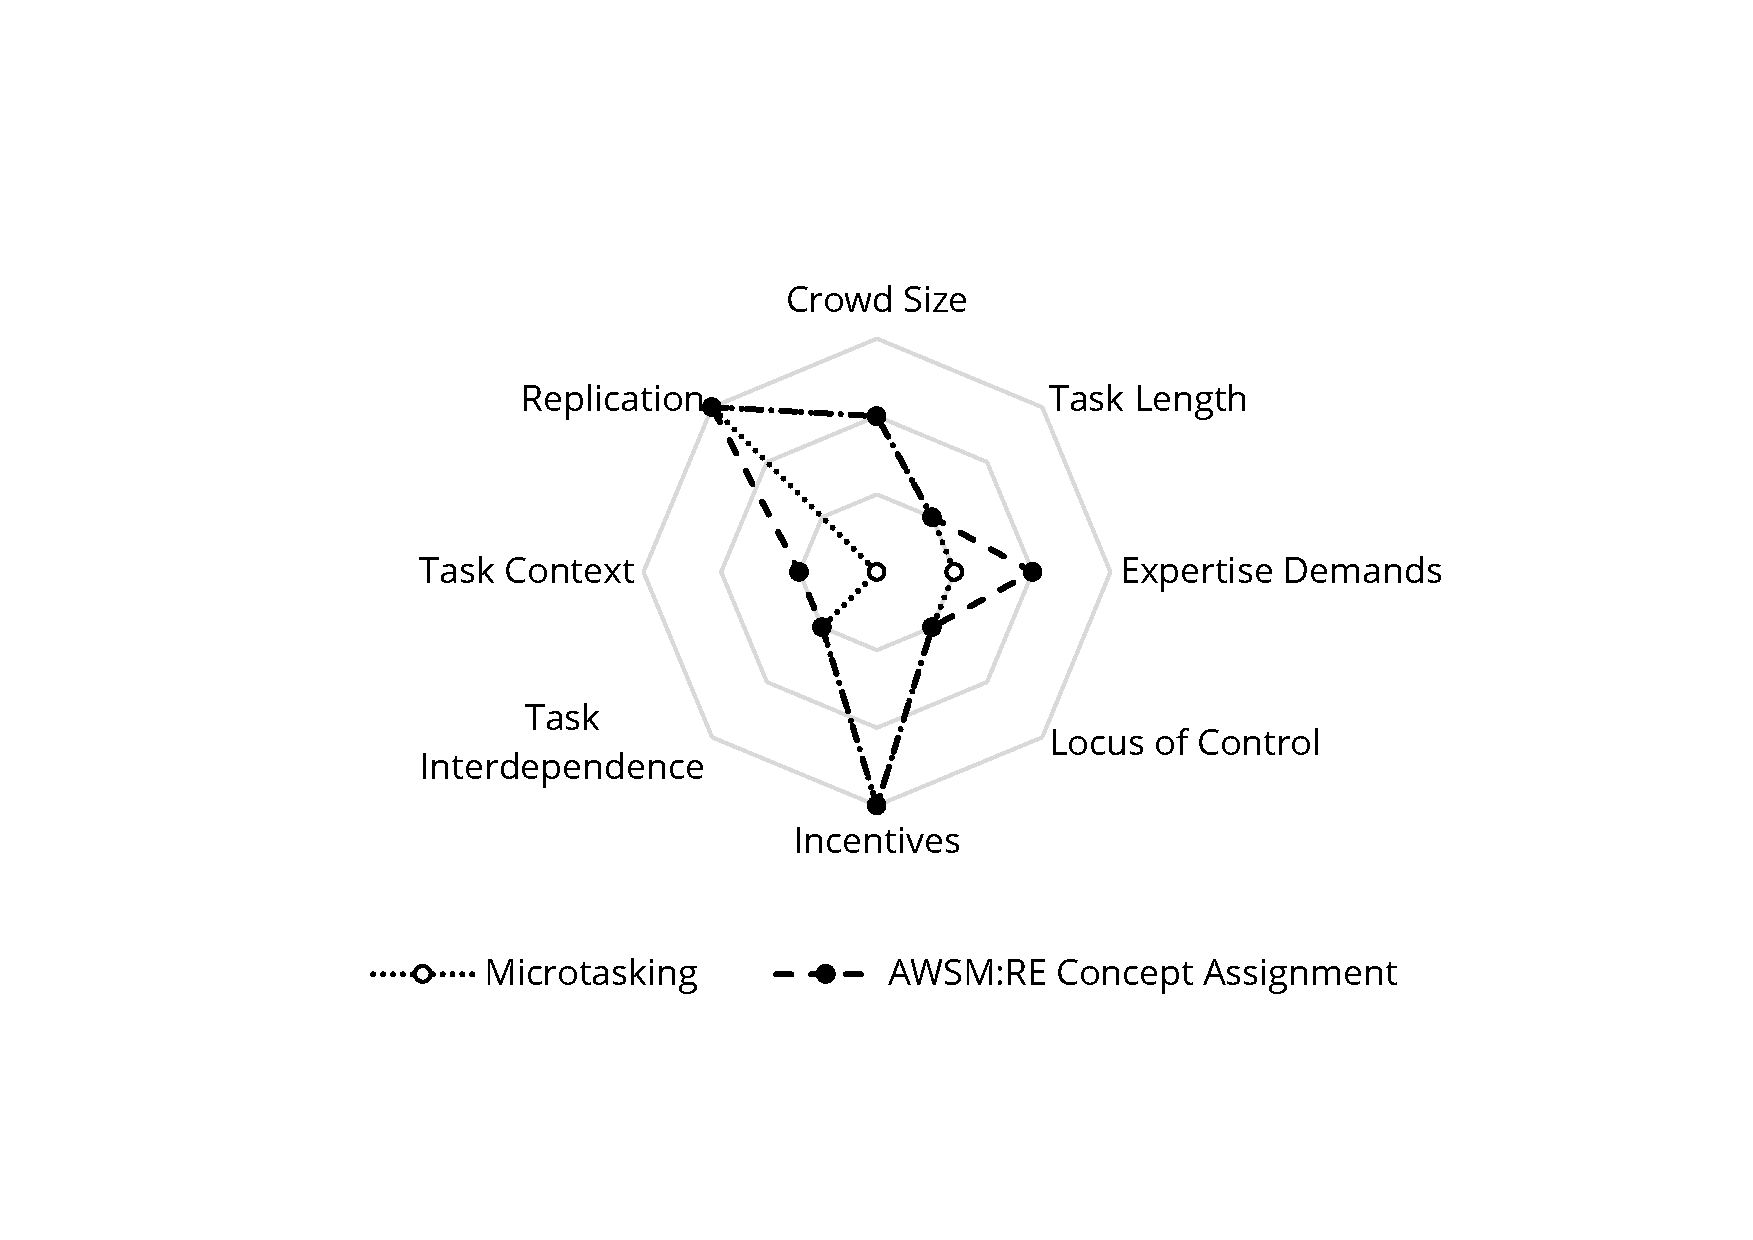
\includegraphics[width=0.75\textwidth]{../figures/spider.pdf}
\caption[Crowd-based Concept Assignment compared to Microtasking]{Crowd-based Concept Assignment compared to Microtasking \autocite{Heil2018CSRE}}\label{fig:awsm.re.crowddimensions}
}
\end{figure}

The resulting localization in the \gls{Crowdsourcing} space places AWSM:RE very close to the established and successful \emph{microtasking} \autocite{Latoza2016} or \emph{marketplace} \autocite{Daniel2018CrowdsourcingQuality} model.
Only two out of eight dimensions do not match exactly: expertise demand and task context of AWSM:RE \gls{Concept Assignment} is higher compared to the low expertise demand and independence of context for typical microtasking tasks.
Due to this high similarity, it is likely that microtasking can be similarly successful for the small, independent, and replicatable classification tasks as for other microtasking applications, benefiting from high worker numbers and parallel execution of tasks.
The potential key benefit of reduced time to market requires two characteristics: work can be broken down into short tasks, and each task must be self-contained with minimal coordination demands \autocite{Latoza2016}.
AWSM:RE meets both of these characteristics.

\begin{figure}[h!]
\hypertarget{fig:crowdprocess}{%
\centering
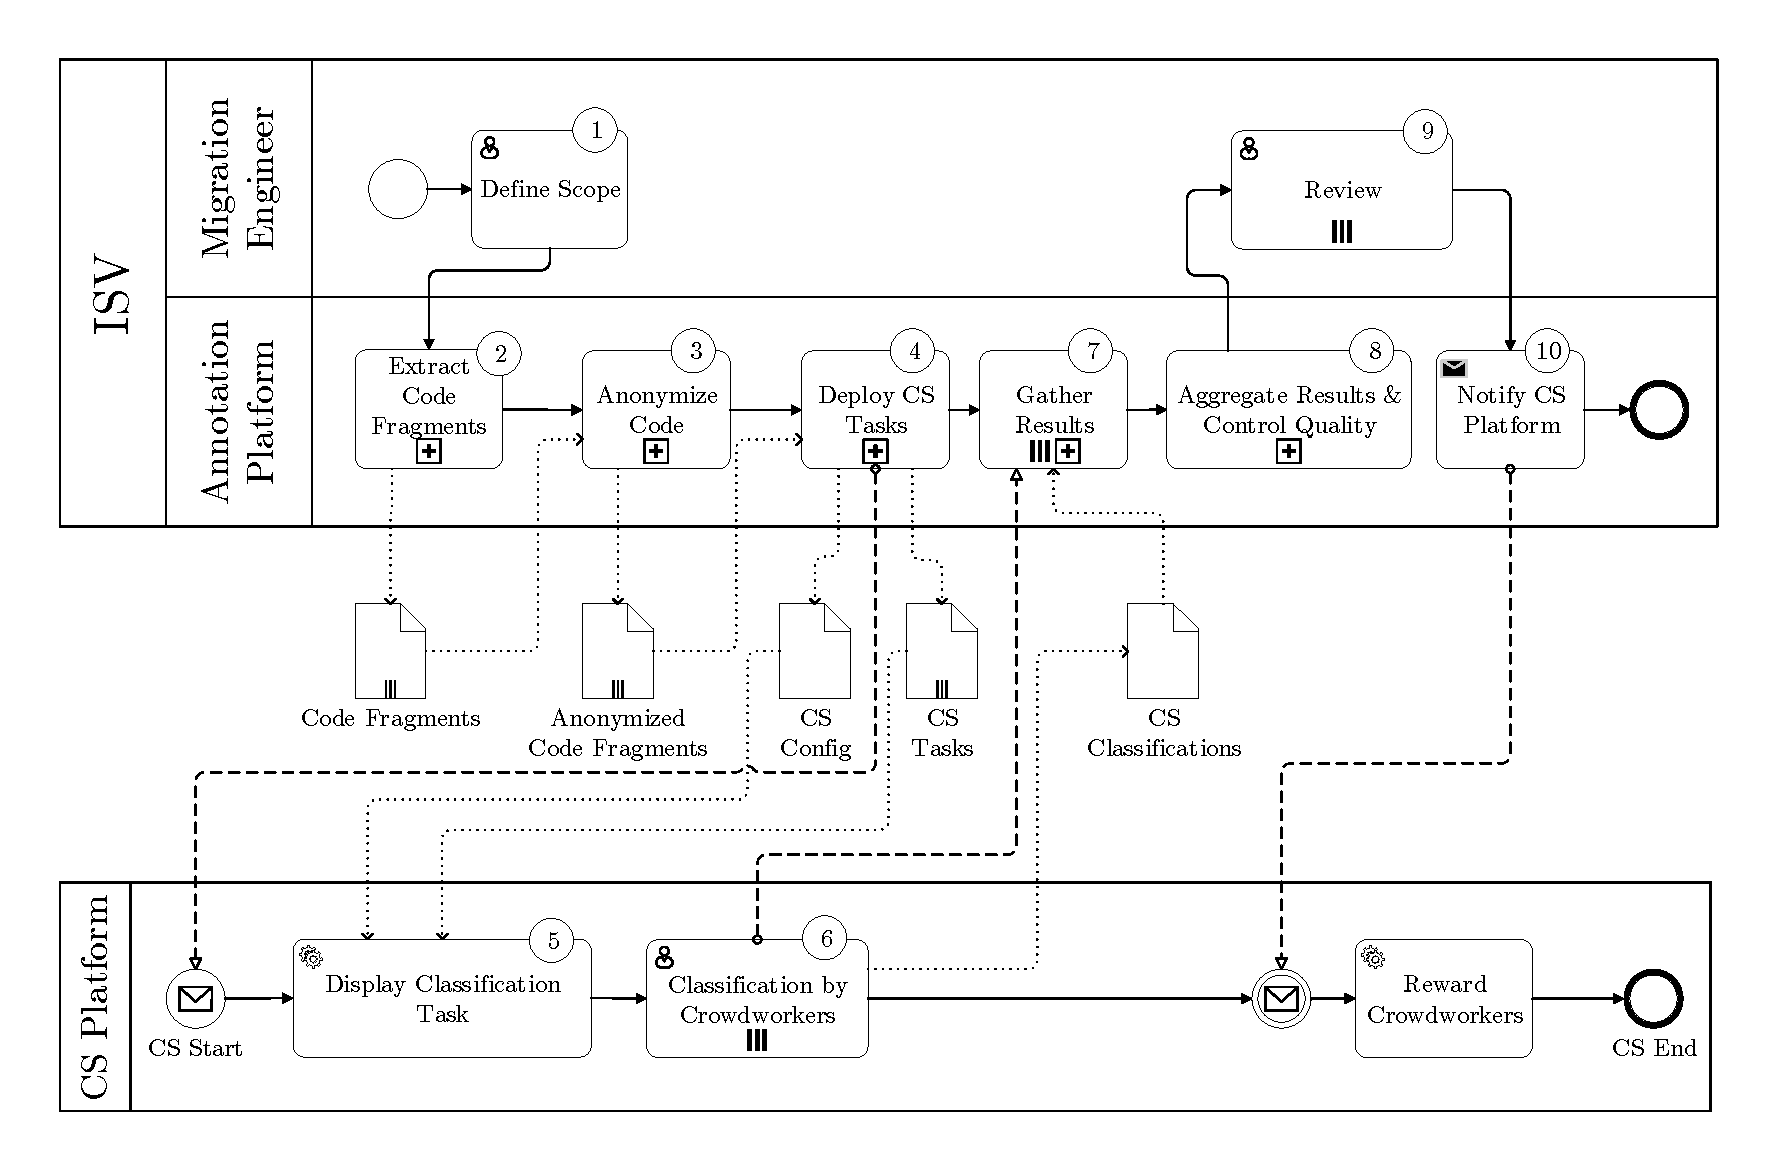
\includegraphics[width=0.99\textwidth]{../figures/crowdprocess.pdf}
\caption[Crowdsourcing-based classification process]{Crowdsourcing-based classification process\\ \autocite[adapted from][]{Heil2019CSRECCIS}}\label{fig:crowdprocess}
}
\end{figure}

For the CSRE extension \autocite{Heil2019CSRECCIS} of AWSM:RE \gls{Concept Assignment}, a suitable \emph{CS Platform} is required, representing a \gls{Crowdsourcing} marketplace to post an open classification call to a crowd.
The adapted process for crowd annotators in \cref{fig:crowdprocess} addresses three main \emph{challenges of the application of \gls{Crowdsourcing} in \gls{Reverse Engineering}} \autocite{Heil2019CSRECCIS}:

\begin{enumerate}
\def\labelenumi{\arabic{enumi}.}
\tightlist
\item
  Automatic Extraction \& Creation of \gls{Crowdsourcing} Tasks from \(B\)
\item
  Balancing Controlled Disclosure of Proprietary Source Code with Readability
\item
  Aggregation of Results and Quality Control
\end{enumerate}

The following subsections outline solutions to address these challenges by detailing the collapsed subprocesses in \cref{fig:crowdprocess}.
The general process is as follows: the \gls{migrationengineer} (1) defines the scope of code to be classified using the filtering capabilities of the Annotation platform described above.
The annotation platform automatically extracts code fragments for classification (2), these are  pre-processed to achieve the intended anonymization properties (3), and the annotation platform deploys classification tasks in the CS Platform (4).
CS Configuration data is passed to the CS Platform to set-up microtasks.
It includes a brief description of the \gls{Concept Assignment} classification task, a URL pointing to the external representation for crowdworkers, the crowdworker selection criteria, and the reward configuration.
Suitable crowdworkers are presented a textual description of the available categories for classification (5), according to the ontology in \cref{sec:representation}.
The interactive external representation of the code fragment to be classified allows the crowdworker to enter his classification (6).
Results are gathered per crowdworker (7), and the classification results are aggregated across the different crowdworkers, and quality control measures are applied (8).
The pre-filtered results are forwarded to the review subprocess in \cref{fig:awsm.re.concept.assignment} and (10) the annotation platform notifies the CS platform to reward the participating crowd workers according to the reward policy (9).

This process was implemented as an extension of \gls{awsmap} for experimentation with CSRE \gls{Concept Assignment} on the bespoke \gls{Crowdsourcing} platform \emph{microWorkers}\footnote{\url{https://microworkers.com/} Retrieved: 6.12.2019} \autocite{Heil2018CSRE,Heil2019CSRECCIS}.
CSRE Management facilities were added for defining the scope, configuring, and starting CSRE projects.
Crowdworker Views (cf.~\cref{fig:crowdview}) were added as external representation for crowd Annotators, showing the information required for the microtasks, and handling token-based authentication of crowdworkers.
Result Analysis Views were added for judging the progress and outcome of CSRE, as in \cref{fig:crowdstatistics} and \cref{fig:crowdrationales}.
The following three subsections describe solutions for the three main challenges of CSRE introduced above.

\vspace{-10pt}
\subsection[Automatic Crowdsourcing Task Extraction \\ \& Creation]{Automatic Extraction and Creation of Crowdsourcing Tasks}
\vspace{10pt}

AWSM:RE \gls{Concept Assignment} was reformulated as classification problem, and the similarity with microtasking was demonstrated.
To apply the microtasking model, self-contained, simple, repetitive, short microtasks are required by automatically dividing \(B\) into \emph{code fragments} for classification through static analysis.
Three \emph{classification task extraction properties} are required: Automation, Legacy Language Support, and Completeness of References \autocite{Heil2018CSRE,Heil2019CSRECCIS}.
\emph{Automation} means that no additional user interaction must be required.
This can be achieved by documentation tools, syntactic analysis tools, or syntax highlighters.
\emph{Legacy Language Support} is important since static analysis is language-specific.
Relevant commonly used\footnote{cf.~\url{https://spectrum.ieee.org/at-work/innovation/the-2018-top-programming-languages} Retrieved: 6.12.2019} \glslink{Legacy System}{legacy} languages, in particular C, \cpp, Java should be supported.
Crowdworkers require sufficient information for classification: control and data flow need to be available.
Thus, \emph{Completeness of References} for the code referenced in a code fragment is required.
A comparative feasibility study with students showed that documentation tools are the best-suited alternative since production-grade implementations exist for most programming languages, they keep track of referenced parts of the source code, and they work entirely automatic.
The implementation of step 2 in \cref{fig:crowdprocess} runs Doxygen\footnote{\url{https://www.doxygen.nl/} Retrieved: 6.12.2019} on \(B\) and parses the generated documentation \glspl{artifact} to identify relevant code fragments and referenced code.

\vspace{-10pt}
\hypertarget{sec:csre.anonym}{%
\subsection{Balancing Controlled Disclosure with Readability}\label{sec:csre.anonym}}
\vspace{10pt}

The open classification call to a potentially large and unknown group of workers means publishing task contents, bearing the risk of uncontrolled use of the code fragments, e.g.~through competitors of the \gls{isv}.
Proper source code anonymization is required to prevent unintended use but must be balanced with the readability of the source code, allowing the crowd to achieve the classification.
This balance is reflected in the following three \emph{anonymization properties}; a suitable approach must: \emph{prevent identification of software provider, software product and application domain}, \emph{maintain control flow and all information relevant for classification}, and \emph{avoid negative impact on readability of the source code} \autocite{Heil2018CSRE,Heil2019CSRECCIS}.
Common code obfuscation techniques are not sufficient as they target readability, but an adapted form of \emph{identifier renaming} is required, extended to all parts of code that contain \emph{identification information} residing in three loci: identifiers, strings, and comments.
\emph{Classification information}, that represents relationships between entities in the code should be kept.

\setlength{\algomargin}{1em} %
\hypertarget{algocf:anonym}{%
\begin{algorithm}
    \DontPrintSemicolon
    \KwIn{Source Code $f \in B$, Platform Specific Model $PSM$, Identifier List $I$}
    \KwOut{Anonymized Source Code}
        $m{(}i{)} = 
        \begin{cases}
        "\text{instance\_of\_}"+m(c) \text{ \textbf{if} }i\text{ instance of }c\\
        \text{genericName}(i)+"\text{\_extends\_}"+ m(s)\text{ \textbf{if} }i\text{ subclass of }s\\
        \text{genericName}(i) \text{ \textbf{else}}
        \end{cases}$\;
        replace Strings in $f$ by $"$String$"$\;
        remove comments from $f$\;
        replace all identifiers $i\in I$ in $f$ with $m(i)$\;
        \Return $f$\;
    \caption{CSRE Anonymization Algorithm}\label{algocf:anonym}
\end{algorithm}}

The CSRE Anonymization Algorithm \autocite{Heil2019CSRECCIS} in \cref{algocf:anonym} implements step 3 in \cref{fig:crowdprocess} and takes a \gls{psm} resulting from the static analysis of the task extraction step and a list of identifiers and automatically generates a replacement mapping for the different types of identifiers.
The mapping represents simple relationships like generalization and class-instance.
We assessed the readability of the anonymized code through a brief experimental validation \autocite{Heil2019CSRECCIS} with employees of an \gls{sme}-sized \gls{isv} who rated the readability of anonymized code fragments on a five-level Likert scale (agreement 1-5 for ''The code is easy to read'').
Code obfuscation ranked near-unreadable (0.7), CSRE Anonymization (3.7) performed slightly better than the naive approach using dictionary replacements (3.2).

\vspace{-15pt}
\subsection{Aggregation of Results and Quality Control}
\vspace{10pt}

Aggregating potentially contradicting results from unknown crowdworkers and ensuring quality is a challenge to be addressed to justify the \gls{isv}'s investment.
Originating in different experience levels of the crowdworkers and fake answers may lead to poor classification precision.
AWSM:RE combines several quality-control design-time (Worker selection, Effective task preparation) and quality control run-time approaches (\emph{Ground truth, Majority consensus}) \autocite{Heil2018CSRE,Heil2019CSRECCIS} to enable the crowdsourcing of \gls{Concept Assignment}, following guidelines for quality control \autocite{Daniel2018CrowdsourcingQuality,Allahbakhsh2013}.
The quality control measures below constitute the \emph{Quality control and results aggregation properties} of CSRE.
CSRE \gls{Concept Assignment} uses \emph{reputation-based worker selection} based on previous crowdworker ratings.
For our experiments on microWorkers.com, we restricted participation to the ``best workers'' group.
\emph{Effective task preparation} comprises clear and unambiguous task description and \emph{defensive design}.
The crowd worker View in \cref{fig:crowdview} provides code fragments and references with syntax highlighting, available \glspl{Concept} to assign and requires min. 50 characters of justification per classification.
This slows down fake contributions and enables filtering and analysis.

The CSRE \emph{compensation policy} is a combination of monetary and non-monetary rewards: quality contributions receive 0.30 USD and a positive rating.
A \emph{Ground Truth} approach is used as runtime quality control: classification tasks with known solution are added to allow calculation of the individual user score \(S(w_i) \in [0,1]\) for each crowd worker \(w_i\in W\) by comparing amounts of correct \(C^+_{w_i}\) and incorrect \(C^-_{w_i}\) classifications as in \cref{eq:userscore}.
This score can be used as weight factor in results aggregation.

\begin{equation}S(w_i) = \frac{|C^+_{w_i}|}{|C^+_{w_i}| + |C^-_{w_i}|}\label{eq:userscore}\end{equation}

CSRE uses \emph{Majority/Group Consensus} for aggregating results from different crowdworkers.
For each code fragment, classifications \(C\subset W \times A\) are tuples of a worker \(w_i \in W\) and an annotation by that worker, expressed as class \(c_k \sim a, a\in A\).
This creates a voting distribution \(V: A \mapsto [0,1]\) for each possible class \(c_k\) as in \cref{eq:voting}.


\begin{equation}V(c_k) = \frac{\sum\limits_{(w,c)\in C | c = c_k} S(w)}{\sum\limits_{(w,c)\in C} S(w)}\label{eq:voting}\end{equation}

\pagebreak
\begin{figure}[h!]
\hypertarget{fig:crowdview}{%
\centering
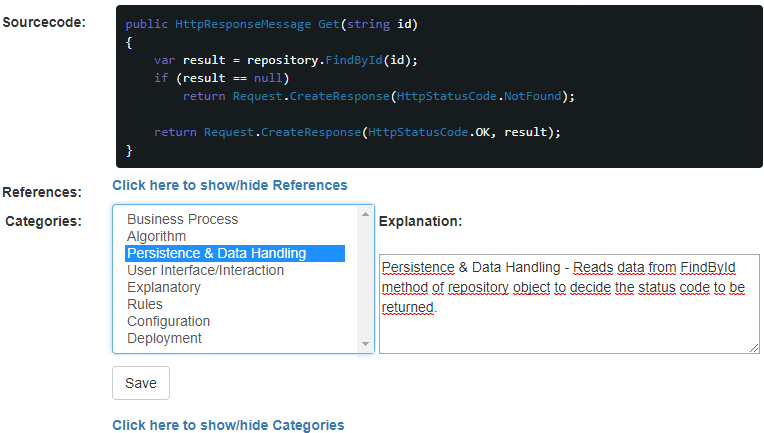
\includegraphics[width=0.95\textwidth]{../figures/screenshots/cw_view.png}
\caption{Crowd Worker View}\label{fig:crowdview}
}
\end{figure}

The aggregated result, the consensual classification \(c^*\) is then calculated from majority consensus as in \cref{eq:consensus}.

\vspace{-10pt}
\begin{equation}c^*=\underset{c \in A}{\operatorname{arg\,max}}\, V(c)\label{eq:consensus}\end{equation}

\vspace{-10pt}
For cases where no clear majority can be found, an overview of result distributions (\cref{fig:crowdstatistics}) and a display of crowdworker rationales (\cref{fig:crowdrationales}) was implemented.

\begin{figure}[h!]
\hypertarget{fig:crowdstatistics}{%
\centering
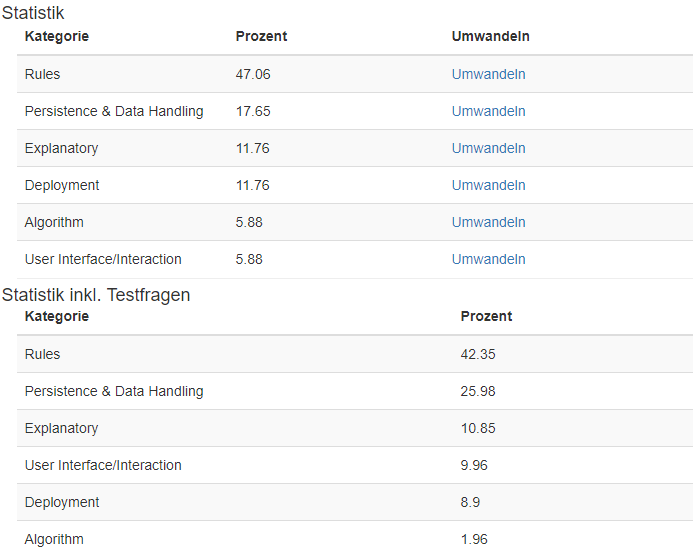
\includegraphics[width=0.75\textwidth]{../figures/screenshots/csre_statistics.png}
\caption{CSRE Statistics}\label{fig:crowdstatistics}
}
\end{figure}

%\vspace{-15pt}
\hypertarget{sec:re.evaluation}{%
\section{Evaluation}\label{sec:re.evaluation}}
\vspace{10pt}

This section evaluates AWSM:RE regarding three aspects.
\Cref{sec:re.evaluation.req} evaluates AWSM:RE against the requirements in \cref{sec:re.requirements}.
Effectiveness and Efficiency are further assessed in detail through experimentation in \cref{sec:csre.experiment}.
\Cref{sec:re.evaluation.objective} revisits research objective \cref{ro:1} and the AWSM:RE research questions in the light of the evaluation results.

\vspace{-35pt}
\hypertarget{sec:re.evaluation.req}{%
\subsection{Assessment of Requirements}\label{sec:re.evaluation.req}}
\vspace{5pt}

This section reports on satisfaction of the requirements for AWSM:RE.

\vspace{-2pt}
\textbf{Effectiveness}. The effectiveness of AWSM:RE for knowledge rediscovery is achieved through specification of a Concept-Assignment-based \gls{Reverse Engineering} technique, which systematically discovers, assigns, and manages knowledge in the \gls{Legacy System}.
A detailed evaluation of results quality is presented in \cref{sec:csre.experiment}.

\textbf{Efficiency}. The efficiency of AWSM:RE is achieved through reformulation of \gls{Concept Assignment} for crowd annotators.
This reduces the resource demand for the \gls{isv} by moving the work from \gls{isv} staff to the crowd.
A detailed evaluation showing the results achievable with very limited financial resources is presented in \cref{sec:csre.experiment}.

\textbf{Expertise}. The expertise requirement is addressed in AWSM:RE by reusing the results of the cognitive process of program comprehension for \gls{Forward Engineering} and by automating decomposition of the \gls{Reverse Engineering} activity of \gls{Concept Assignment} into microtasks that are solved leveraging crowd expertise.
While \gls{Web Migration} activities always pose some expertise demands for \gls{isv} staff in new fields, AWSM:RE conditionally meets the expertise requirement as it is a method that is feasible with available staff assuming a general understanding of software engineering activities and learning capability.

\textbf{Integration}. Integration is one of the core design maxims of AWSM:RE.
\Cref{sec:re.conceptual.process} has presented the integration of AWSM:RE processes into ongoing development and maintenance activities following the continuous \gls{Reverse Engineering} paradigm and \cref{sec:re.impl.integration} presented the implementation of the integration aspects in the \gls{awsm} Toolsuite through connection of \gls{awsm}AP with core components of \glspl{isv}' development environment Thus, AWSM:RE meets the integration requirement.

\textbf{Knowledge Management}. The knowledge discovered through AWSM:RE is represented based on open \gls{web} standards like \gls{owl}, \gls{rdf} and \gls{w3c}{oa} as described in \cref{sec:representation} and is available for integration with different model-driven or non-model-driven methods through its external representation for subsequent human use via the \glslink{web}{Web}-based user interface and for system use via the queryable interface based on SPARQL and Querying Support as described in \cref{sec:representation}.
Thus, AWSM:RE meets the knowledge management requirement.

\vspace{-15pt}
\hypertarget{sec:csre.experiment}{%
\subsection{Experimental Evaluation of CSRE}\label{sec:csre.experiment}}
\vspace{10pt}

As the idea of CSRE, i.e.~application of the \gls{Crowdsourcing} paradigm to \gls{Reverse Engineering}, is novel, we conducted evaluation experiments \autocite{Heil2019CSRECCIS}.
The results provide a basis for assessing efficiency and effectiveness of AWSM:RE for crowd Annotators.
Furthermore, the analysis aimed at exploring the suitability of crowdworkers for CSRE and exploring crowdworker behaviors.

\textbf{Setup}. The automatic task extraction described above was used to pre-process the codebase of BlogEngine.NET\footnote{\url{http://www.dotnetblogengine.net/} Retrieved: 6.12.2019}, from which 10 code fragments were randomly selected.
Length distribution of the fragments was between 7 and 57 \gls{loc}, average 25.4 \gls{loc}.
The set of classes \(\overline C\) was formed from the 8 domain knowledge types of the \gls{sckm} ontology \cref{fig:ontology} as \glspl{Concept} to be assigned to the fragments.
All 10 fragments were manually classified so that the \emph{test dataset} consisted of 10 classified code fragments which formed the ground truth as baseline for assessing crowdworker results.
Experiments were run on the crowd-extended \gls{awsmap} with microWorkers as \gls{Crowdsourcing} platform, restricted to the ``best workers'' group.

\textbf{Procedure}. A classification campaign was run for 14 days between March 14th and March 28th 2017 with 0.30 USD -- platform average at this time -- as financial reward per 3 classifications.
The crowdworkers were presented a detailed explanation of the classification task and the available classifications and then used the Crowdworker View to perform the classifications.
The integration mechanism of microWorkers for external \glspl{Web Application} is an IFrame.
3 code fragments were randomly selected from the pool of 10 fragments available and classified by the crowdworkers, who could repeat the classification until less than 3 fragments not classified by them were available.
To observe the crowdworkers' behavior, \texttt{focus} and \texttt{blur} events in the Crowdworker View were used to track the time spent.

\begin{table}[hbt]
  \caption[CSRE Experimental Results]{CSRE Experimental Results \autocite{Heil2019CSRECCIS}}
  \label{tbl:csre-results}
  \centering
    \begin{tabularx}{0.57\textwidth}{ l c c c c c c c c l }
        &  \multicolumn{8}{l}{\textbf{Categories}} \\
        \textbf{CF} & \textbf{1} & \textbf{2} & \textbf{3} & \textbf{4} & \textbf{5} & \textbf{6} & \textbf{7} & \textbf{8} & \textbf{Consensus}\\
    \hline
    A & 1 & \cellcolor{lightgray}\textbf{14} & 4 & 1 & 1 & 1 & 1 & 1 & Algorithm\\%HashPassword
    B & 0 & 1 & 3 & 0 & 0 & \cellcolor{lightgray}\textbf{12} & 0 & 0 & Rule\\%CanPublish
    C & 3 & 0 & \cellcolor{lightgray}\textbf{4} & 1 & 0 & 1 & 0 & 0 & Persistence\\%FillCustomFields
    D & 2 & 5 & \cellcolor{lightgray}\textbf{6} & 3 & 0 & 5 & 2 & 0 & Persistence\\%Get
    E & 4 & 2 & 1 & \cellcolor{lightgray}\textbf{9} & 2 & 0 & 3 & 1 & UIX\\%LoginUser_OnAuthenticate
    F & 0 & 0 & 3 & 0 & 1 & 6 & \cellcolor{lightgray}\textbf{7} & 2 & Config\\%Initialize
    G & 3 & 1 & 1 & 2 & \cellcolor{lightgray}2 & \textbf{6} & 0 & 0 & Rule\\%GetWebResponse
    H & 0 & 2 & \cellcolor{lightgray}\textbf{12} & 2 & 4 & 3 & 2 & 2 & Persistence\\%CreateRole
    I & \cellcolor{lightgray}0 & 1 & 3 & 1 & 2 & \textbf{8} & 0 & 2 & Rule\\%FillCategories
    J & 2 & 2 & \textbf{4} & 0 & 1 & 2 & \cellcolor{lightgray}1 & \textbf{4} & Persistence/Deployment\\%CreateProvider
    \hline
    \end{tabularx}
\end{table}
\setcounter{table}{1}

\textbf{Experimental results and descriptive statistics}. 34 unique crowdworkers participated in the experiment, contributing 187 classifications on our test dataset.
The results are shown in \cref{tbl:csre-results}.
On average, 16 crowdworkers created 18.7 classifications per code fragment.
\(CF\) are the ten code fragments, Consensus indicates the result of the consensus voting.
The numbers of classifications per category are stated in the categories cells.
Bold values are the maxima, which are the basis for the majority consensus.
Grey background marks the correct classification of the code fragment.
Descriptive statistics of the results are shown in \cref{tbl:csre-statistics}, where \(|C|\) is the number of classifications and \(|W|\) the number of crowdworkers.
Note that the crowdworker and classification numbers differ due to multi-selections.
The code fragment length in \gls{loc} is stated in \(l\), \(\Sigma t\) reports the overall time spent, \(\overline t\) is the average time.
Times are reported in seconds.
The error rate \(f_e\) (cf.~\cref{eq:errorrate})

\begin{equation}f_e = \frac{|C^-|}{|C|}\label{eq:errorrate}\end{equation}

is the ratio between false classifications \(C^-\) and all crowdworker classifications \(C\) of a code fragment.
In order to investigate indicators of (dis-)agreement between individual crowdworkers for quality control, \cref{tbl:csre-statistics} includes Entropy \(E\) (cf.~\cref{eq:entropy})

\begin{equation}E = - \sum\limits^k_{I=1}f_i \lg f_i\label{eq:entropy}\end{equation}

and normalised Herfindahl dispersion measure \(H^*\) (cf.~\cref{eq:herfindahl})

\begin{equation}H^*=\frac{k}{k-1}\left(1-\sum\limits_{i=1}^{k}f_i^2\right)\label{eq:herfindahl}\end{equation}

from the relative frequencies \(f_i\) of the classifications in the \(k=8\) classes.
\(E\) And \(H^*\) both indicate disorder/dispersion among the crowdworkers: unanimous classifications yield \(E=H^*=0\).
The higher the disagreement, the more different classifications, the closer \(E\) And \(H^*\) get to 1.
Thus, they are used as indicators of classification certainty in the following analysis.
\Cref{fig:crowdrationales} shows a subset of the rationales provided by crowdworkers to justify their classifications.

\begin{table}[hbt]
  \caption[CSRE Experiment Descriptive Statistics]{CSRE Experiment Descriptive Statistics \autocite{Heil2019CSRECCIS}}
  \label{tbl:csre-statistics}
  \centering
    \begin{tabularx}{0.52\textwidth}{ ll l l l l l l l }
        \textbf{CF} & $\boldsymbol{|C|}$ & $\boldsymbol{|W|}$ & $\boldsymbol{l}$ & $\boldsymbol{\Sigma t}$ & $\boldsymbol{\overline{t}}$ & $\boldsymbol{f_e}$ & $\boldsymbol{E}$ & $\boldsymbol{H^{*}}$ \\ %& \textbf{Consensus}\\
    \hline
    A & 24 & 19  & 18 & 2822 & 122 & 0.4167 & 0.6113 & 0.6906 \\ %& Algorithm\\%HashPassword
    B & 16 & 16  & 20 & 2531 & 158 & 0.25 & 0.3053 & 0.4427 \\ %& Rule\\%CanPublish
    C & 10 & 10  & 40 & 1128 & 112 & 0.6 &0.6160 & 0.8 \\ %& Persistence\\%FillCustomFields
    D & 23 & 21  & 8  & 3033 & 131 & 0.7391 & 0.7402 & 0.8948 \\ %& Persistence\\%Get
    E & 22 & 18  & 7  & 2580 & 117 & 0.5909 & 0.7228 & 0.8448 \\ %& UIX\\%LoginUser_OnAuthenticate
    F & 19 & 15  & 28 & 2857 & 150 & 0.6316 & 0.6146 & 0.8064 \\ %& Config\\%Initialize
    G & 15 & 13  & 57 & 3225 & 215 & 0.8667 & 0.6891 & 0.8395 \\ %& Rule\\%GetWebResponse
    H & 25 & 21  & 24 & 5249 & 209 & 0.52 & 0.6541 & 0.7893 \\ %& Persistence\\%CreateRole
    I & 17 & 13  & 40 & 1917 & 112 & 1 & 0.6504 & 0.7920 \\ %& Rule\\%FillCategories
    J & 16 & 14  & 12 & 3393 & 212 & 0.9375 & 0.7902 & 0.9115 \\ %& Pers./Depl.\\%CreateProvider
    \hline
    \end{tabularx}
\end{table}

\begin{figure}[h!]
\hypertarget{fig:crowdrationales}{%
\centering
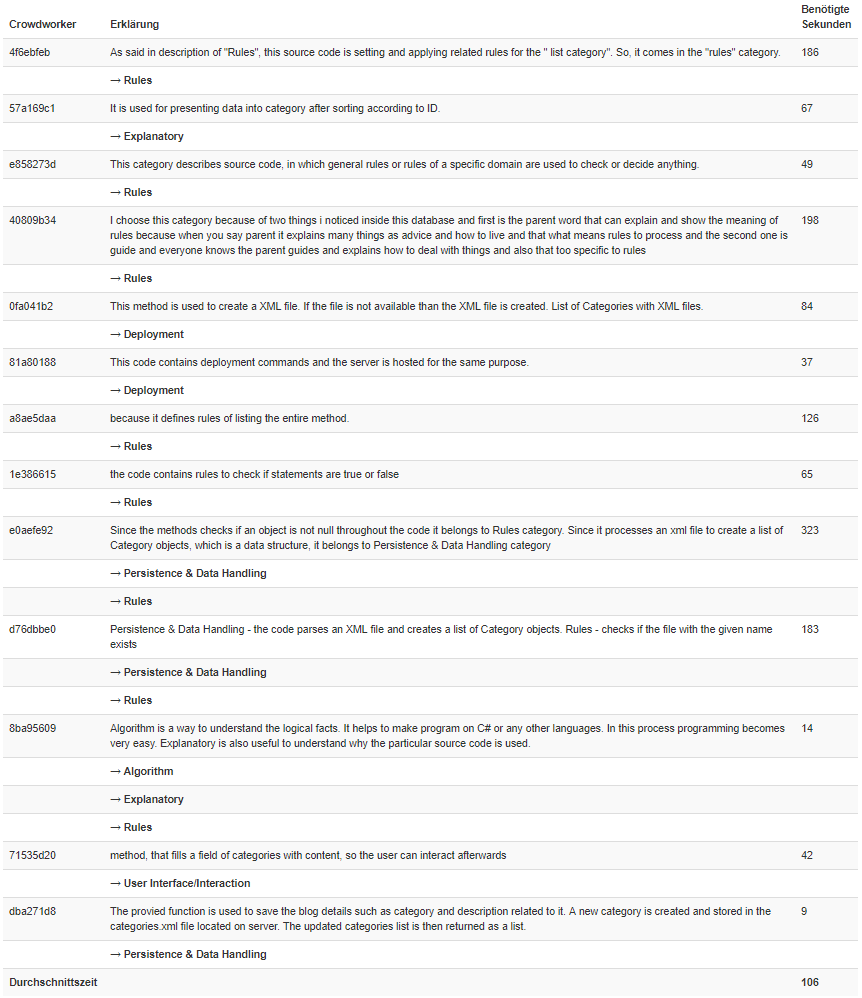
\includegraphics[width=0.99\textwidth]{../figures/screenshots/csre_cw_answers.png}
\caption[CSRE Results View]{CSRE Results View in Annotation Platform, showing classification justifications provided by crowd workers during the experiment and required classification times}\label{fig:crowdrationales}
}
\end{figure}

\textbf{Quality and classification certainty analysis}. An average error rate of 0.655 seems high at first.
However, through majority consensus 7 of 10 code fragments were classified correctly.
The minimum error rate was .25 on fragment B and the maximum 1 for fragment I.
Provided a small expertise variation of the participating crowd workers, this indicates differences in the difficulty (fragment I was one of the longest) and the understanding of the categories.
Rule was the \gls{Concept} most frequently assigned (23.5\%), Persistence \& Data Handling (21.9\%) second, was Deployment the least selected (5.3\%).
No majorities were achieved for the Business Process and Explanatory \glspl{Concept}, indicating that they might not be described clear enough for the crowdworkers.
All other categories were correctly classified by the respective majorities.

Averages of entropy and Herfindahl dispersion measure are \(\overline E = 0.639\) and \(\overline{H^*} = 0.757\), their minima co-occur with minimal error rate, their maxima with the second-highest \(f_e\).
\Cref{fig:crowd-errors} shows \(E\) and \(H^*\) plotted over \(f_e\) and their fit to a squared regression.
There is a significant (\(\alpha=0.05\)) positive correlation (Spearman's \(\rho=0.649\), \(p=0.049\)) between \(f_e\) and \(H^*\) and between \(f_e\) and \(E\) (\(\rho=0.6\), \(p=0.073\)), significant at \(\alpha=0.1\).
Under the peaks at \(f_e=0.8)\), that means that \(E\) and \(H^*\) can be used as classification thresholds, i.e.~the more crowd workers voting a \gls{Concept}, the less likely it is a wrong classification.
No clear majorities for wrong classifications were observed, supporting the fundamental \gls{Crowdsourcing} principle \emph{``wisdom of the masses''} and the majority consensus assumption, that majorities are indicative of correct answers.

\begin{figure}[h!]
\hypertarget{fig:crowd-errors}{%
\centering
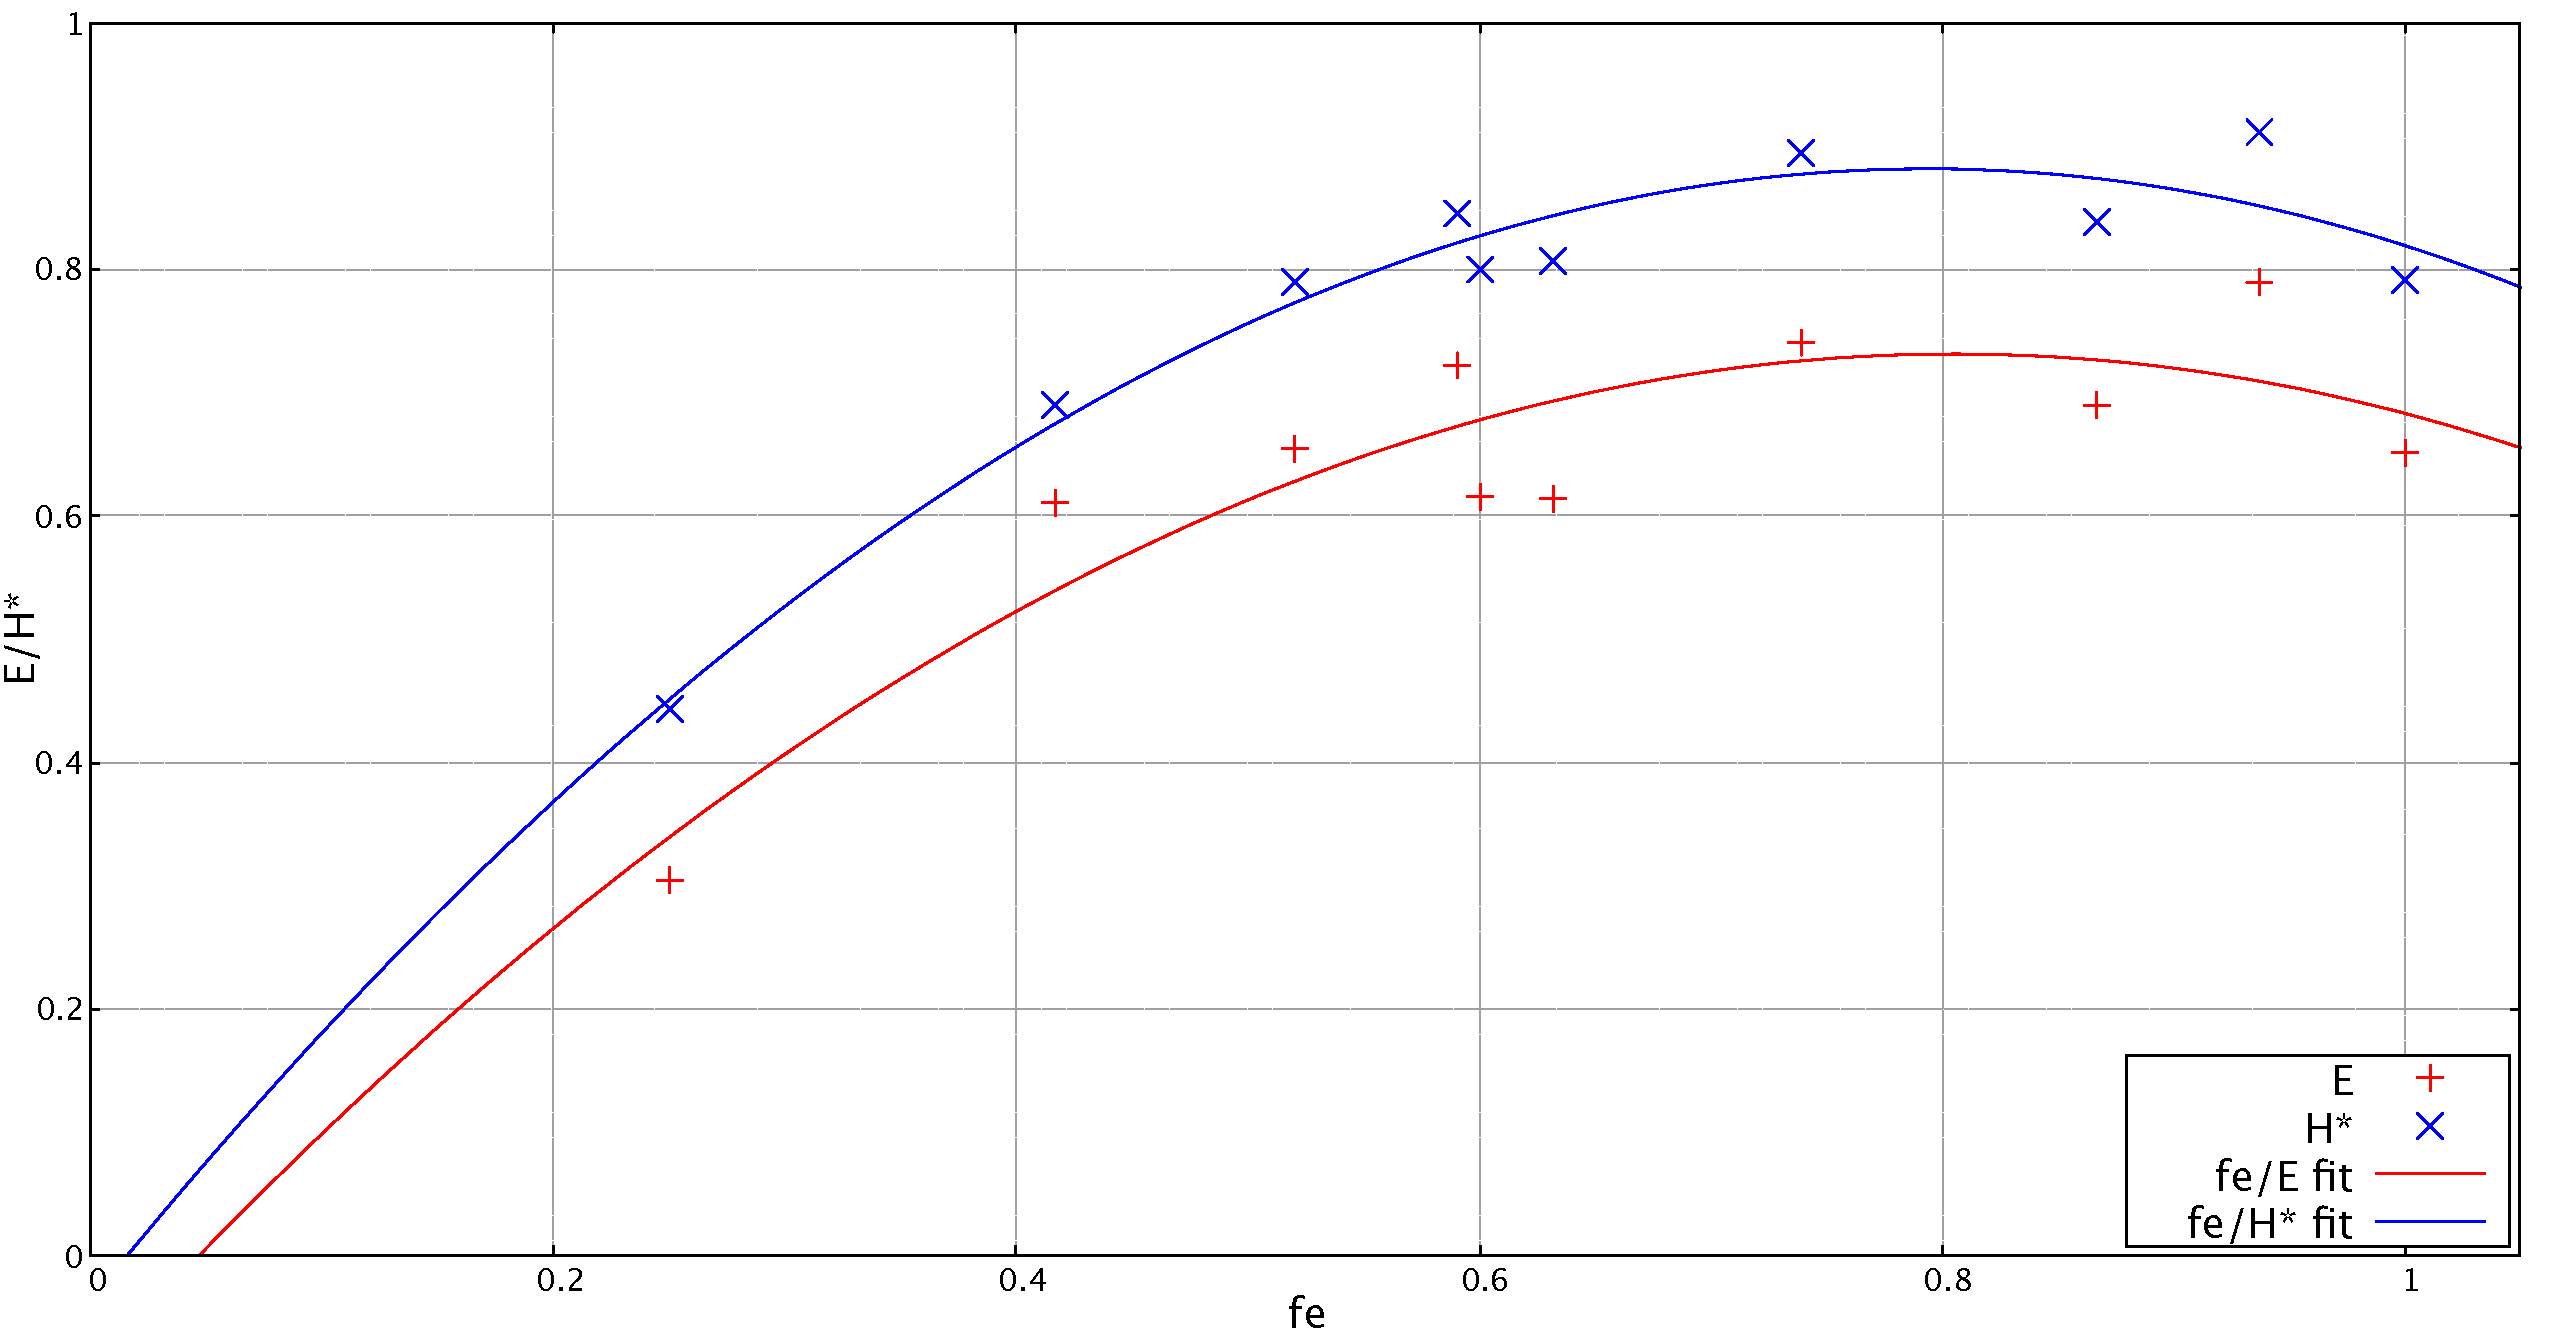
\includegraphics[width=0.85\textwidth]{../figures/crowd-errors.pdf}
\caption{Error Rate and Entropy/normalized Herfindahl measure}\label{fig:crowd-errors}
}
\end{figure}

No correlation between length of code fragments and classification time was found, indicating the influence of other variables such as different levels of difficulty/clarity of the classification.
Considering correctness, correct classifications showed fewer time outliers\footnote{we use \(Q3 + 1.5 \text{ IQR}\) as outlier threshold} than wrong classifications.
A likely interpretation is that longer classification time and explanations are indicative of uncertainty, leading to wrong classifications in most observed cases.
Most outliers in \cref{fig:scatterplots-c} belong to \emph{Persistance \& Data Handling}, the second most frequently voted, and indicating that the formulation of this \gls{Concept} is not precise enough.

\textbf{Crowdworker behavior analysis}. Crowdworker behavior was analyzed through consideration of the distributions of time and explanation length, as well as derived length-time ratio and average explanation similarity per worker, as shown in \cref{fig:csre-boxplots}.
Time median was \(\tilde t=\) 117.5s, but the observed times varied widely.
The interquartile range was at IQR = 143.25s, while upper outliers reached near half an hour (1606s).
The relatively low times (Q1 at 65s, min time 6s) show the microtask nature but also point to fake contributions as described below.
However, longer times do not imply better accuracy: all but one time outlier in \cref{fig:csre-boxplots-a} belonged to \(C^-\).
The results of one particular crowdworker showed suspiciously identical time measurements (3x14s, 3x33s, 3x515s) and identical explanations in all three groups, most likely resulting from the use of a record-and-replay script.

Explanation lengths in \cref{fig:csre-boxplots-b} range from 51 to 1017 characters (median
\(\tilde{d}\)=119) and are relatively close (IQR=100.5) to the minimal threshold of 50 chars of explanation.
Most of the crowdworkers wrote rather short explanations in short time
This can be seen by considering the lower quartile of 76.25 characters and the outliers for time and length only appearing above the third quartile.
\Cref{fig:csre-scatterplots} shows the values for explanation length and time in relation, with correct classifications in green and wrong in red.

\begin{figure}[h]
\centering

\subfloat[Classification Time (s)]{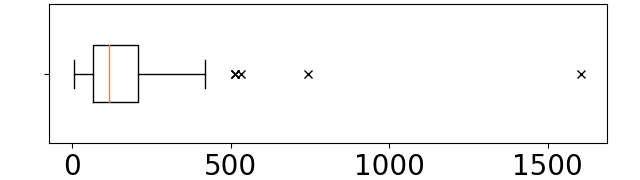
\includegraphics[width=0.49\textwidth]{../figures/csre/boxplot_times.png}\label{fig:csre-boxplots-a}}
\subfloat[Explanation Length (char)]{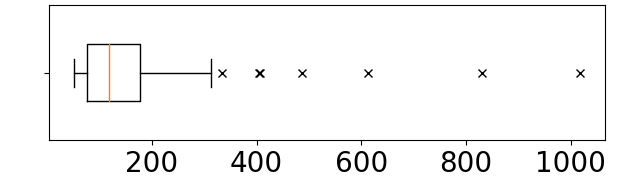
\includegraphics[width=0.49\textwidth]{../figures/csre/boxplot_length.png}\label{fig:csre-boxplots-b}}

\subfloat[Length-Time Ratio (cps) cut at 30]{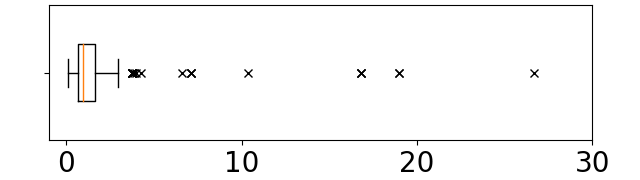
\includegraphics[width=0.49\textwidth]{../figures/csre/boxplot_cps_cut30.png}\label{fig:csre-boxplots-c}}
\subfloat[Avg. Explanation Distances]{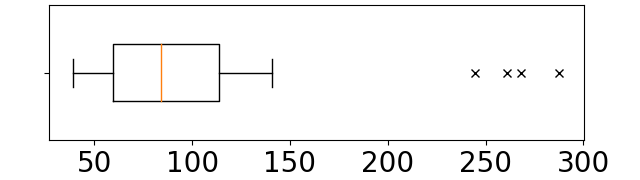
\includegraphics[width=0.49\textwidth]{../figures/csre/boxplot_leven.png}\label{fig:csre-boxplots-d}}

\caption[Classification Time, Explanation Length: 1-dimensional Distributions]{Classification Time and Explanation Length: 1-dimensional Distributions \autocite{Heil2019CSRECCIS}}
\label{fig:csre-boxplots}
\end{figure}

\textbf{Analysis of fake contributions}. Cheating is an issue for the quality of \gls{Crowdsourcing} \autocite{Daniel2018CrowdsourcingQuality,Allahbakhsh2013}.
Observations in time and explanation length distributions revealed that some crowdworkers tried to gain the reward quickly through fake contributions.
To identify very fast classifications, length-time ratio\footnote{measured in characters per second (cps)} was calculated.
As shown in \cref{fig:csre-boxplots-c}, within a range of 0.13 to 61.2 cps, the majority of values is distributed very closely (IQR 0.96 cps) around a median of 0.94 cps.
Analysis of the 20 outliers showed that they are likely to have copied texts.
These copies were most often copies of own previous explanations and in some cases from the task description.
As the measured time does not only include time for typing the rationales in the explanation field, but also source reading, understanding, deciding and selecting the classification, very high length-time ratios were only reachable if little time was spent for thorough consideration, as evident by only 4 of 20 outliers belonging to \(C^+\).
In any case, speeds are not likely to exceed the upper level of 16 cps measured at competitions\footnote{cf.~\url{http://www.intersteno.org/} Retrieved: 6.12.2019}.
However, 7 crowdworkers exceeded this level.
Manual analysis of explanations provided by the outliers determined the fastest worker not to copy text and to classify correctly at approx.
6.6 cps.
The upper quartile at 1.63 cps, the vast majority of crowdworkers produced results in reasonable time.

To further identify workers completing the tasks very quickly through copying, average similarity of explanations per user was calculated using pairwise Levenshtein distance.
The averages range from 39 to 287 and are concentrated (IQR=54.5) around a median of 83.8
(cf.~\cref{fig:csre-boxplots-d}).
Identical copies (distance 0) were recorded from 10 of 34 (29.4\%) workers, but the minimum Levenshtein average of 39 indicates that crowd workers did not exclusively copy.
Normalized with \(\overline l\), two workers had even less than 50\% relative changes, copying most explanations with only minor adaptions.
Manual inspection of responses showed that 3 of 34 exclusively put code in their explanations, indicating a wrong understanding of the task.

\begin{figure}[h]
\centering

\subfloat[correct and wrong]{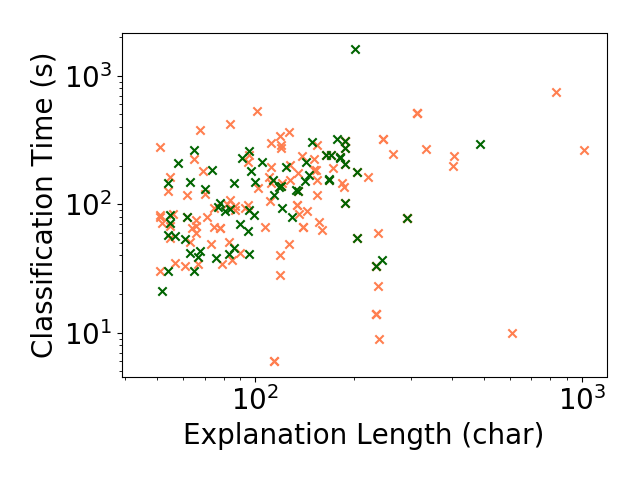
\includegraphics[width=0.52\textwidth]{../figures/csre/timeVSlength_gr.png}\label{fig:scatterplots-a}}

\subfloat[correct only]{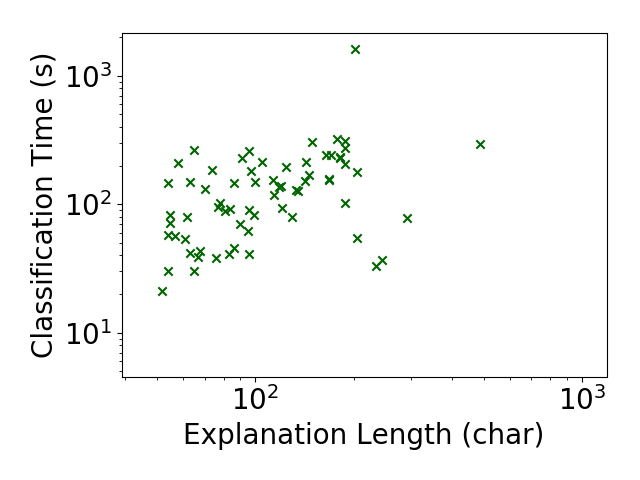
\includegraphics[width=0.49\textwidth]{../figures/csre/timeVSlength_g.png}\label{fig:scatterplots-b}}
\subfloat[wrong only]{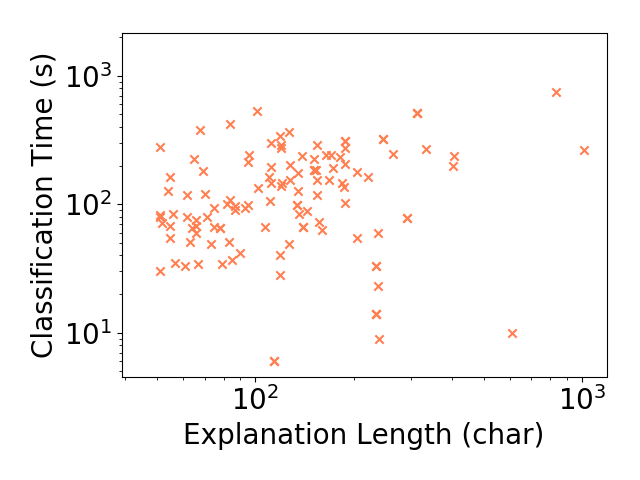
\includegraphics[width=0.49\textwidth]{../figures/csre/timeVSlength_r.png}\label{fig:scatterplots-c}}

\caption[Classification Time, Explanation Length]{Classification Time and Explanation Length (log scaled) \autocite{Heil2019CSRECCIS}}
\label{fig:csre-scatterplots}
\end{figure}

\textbf{High crowdworker commitment}. In contrast to the negative cases analyzed in detail above, also very thorough workers have been observed: Fragment J was split-voted as Persistence/Deployment assignment.
The explanations argued that J is related to persistence because the fragment is part of a class related to persistence.
This observation was
fascinating, because our dataset did not include the code of the surrounding class.
Thus, several crowd workers looked up the sample on the \gls{web} and also read the surrounding parts from an external source in order to classify.
This level of active commitment and investment of time by the crowdworkers
to complete their task was positively surprising.

\textbf{Threats to Validity}. The experiments conducted in the context of this thesis all comprise an analysis of threats to validity.
This analysis is structured according to the three different types of validity: construct validity, internal validity, and external validity.
\emph{Construct validity} is the validity of the experimental design, determining whether the measured indicators are appropriate for the intended construct as abstraction of the latent variables.
\emph{Internal validity} is the validity of cause-effect relationships observed in an experiment established by ruling out alternative explanations as originating from systematic error.
\emph{External validity} is the validity of generalization based on the results of an experiment.
\autocite{Creswell2014ResearchDesign}

\emph{Construct validity} of this experiment is threatened by the explanations for the available classes in \(\overline C\), which may have lead to differences in the understanding across crowd workers.
However, these differences are also expected when operationalizing the CSRE method and are addressed by the multiple redundancy of classification results.
Another threat to construct validity is the relatively hidden possibility to assign several classes.
As only very few crowdworkers used this functionality, their impact on the results is limited.
The third threat to construct validity are random classifications.
These were, however, expected and addressed both through the quality control measures and our detailed analysis of fake contributions showing, that the vast majority of contributions was appropriate and that the quality control measures are effective in mitigating the effects of fake contributions.
The measured error rates are valid indicators of the desired classification quality required for \gls{isv} usage, as higher errors lead to more effort for checking the results, lowering the advantage of employing \gls{Crowdsourcing}.

\emph{Internal validity} of this experiment is threatened through potential subjective biases.
This is addressed through a purely tool-based interaction with the test subjects, i.e.~the crowdworkers.
There was no interaction between the researchers and the test subjects; all test subjects used the exact same experimental setup, which was unchanged throughout the entire experimental timespan.
There were no hints towards the correct or expected classification result in the user interface, and the test objects, i.e.~the code fragments, were randomly assigned to the test subjects, avoiding the bias of improved results through learning over time on specific code fragments.
The 14 days experimentation timespan reduces the test subject selection bias, allowing persons of different time-availability, e.g.~weekend-only vs.~weekdays, business hours vs.~evening, to participate.

\emph{External validity} of the experiment is threatened through limitations in the generalizability of results.
The main factor is the test subjects who conducted the experiment.
As described above, the two weeks experimentation period reduced test subject selection bias, so that the 34 participating crowdworkers from the microWorkers \gls{Crowdsourcing} platform can be considered sufficiently representative of the quality characteristics for crowdworkers on this general-purpose \gls{Crowdsourcing} platform.
While the results cannot be generalized to arbitrary platforms, we would expect an even better quality on a dedicated software development platform such as topcoder\footnote{\url{https://www.topcoder.com} Retrieved: 6.12.2019}.
The test objects, i.e.~the code fragments, limit generalisability of results since they are selected from one specific technology and platform, C\# and Microsoft .NET.
However, we expect results for other technologies and platforms used in \glspl{Legacy System} such as Java Swing, C/\cpp \gls{mfc} to be at least similar due to higher popularity\footnote{cf.~TIOBE Index \url{ https://www.tiobe.com/tiobe-index/} Retrieved: 6.12.2019} and therefore greater availability of crowdworkers experienced in this technological base.

\textbf{Conclusion of CSRE Experimentation}. In spite of the cases of low quality and fake contributions reported
above, the CSRE quality control measures proved robust enough to yield 70\% overall correctness.
The experiment has shown that the expertise level of the best crowd workers group on \gls{Crowdsourcing} platform microWorkers in combination with CSRE quality control is sufficient to perform the \gls{Reverse Engineering} classification activity and produce decent results.
The overall correctness of 70\% is a good result similar to what can be achieved by a single expert performing the same task.
However, with less than 20 USD expenses for classifying the ten code fragments, \gls{Crowdsourcing} is a significantly
more cost-effective solution.
The results indicate that \gls{Crowdsourcing} can be applied to perform AWSM:RE \gls{Concept Assignment} reformulated as classification problem when it is automatically broken down into microtasks, and the process is guided by CSRE quality control methods.
CSRE \gls{Concept Assignment} defines a novel manual knowledge rediscovery approach reducing the resource demand for \glspl{isv} through \gls{Crowdsourcing}.
Thus, the requirements effectiveness and efficiency requirements from \cref{sec:re.requirements} are met.

%\vspace{-15pt}
\hypertarget{sec:re.evaluation.objective}{%
\subsection{Research Results}\label{sec:re.evaluation.objective}}
\vspace{5pt}

The research objective addressed by this chapter, \cref{ro:1}, to enable identification and management of existing knowledge in legacy source code with limited resources and lack of \gls{Web Engineering} expertise, is achieved.
The effectiveness and efficiency of the AWSM:RE Method for knowledge discovery have been demonstrated and detailed through experimentation, its feasibility with limited resources and lack of expertise is achieved through Crowdsourcing and Integration with ongoing development and its Knowledge Management functionality based on stakeholder-specific user interfaces, and queryable standards-based representations were presented.
AWSM:RE RQ1 was answered through the knowledge discovery technique defined in \cref{sec:re.conceptual.process}, its integration into ongoing development and its realization as crowdsourced activity.
AWSM:RE RQ2 was answered through the introduction of the novel Crowdsourced Reverse Engineering strategy presented in \cref{sec:csre}.
AWSM:RE RQ3 was answered through specification of the Annotation Platform  presented in \cref{sec:extraction.platform}.

\vspace{-20pt}
\hypertarget{sec:re.summary}{%
\section{Summary}\label{sec:re.summary}}
\vspace{7pt}

This chapter presented the \gls{awsm} \gls{Reverse Engineering} method, which facilitates problem and solution domain knowledge rediscovery for \glspl{isv} with limited resources, specifying a novel crowdsourced \gls{Concept Assignment} strategy.
AWSM:RE integrates with ongoing development and providesa queryable open \gls{web} standards-based knowledge representation to facilitate integration with other \gls{Web Migration} methods.
The AWSM:RE techniques and their implementation in the Annotation Platform have been described.
Experimental evaluation has shown the feasibility of the approach, quality of its results, and low related cost and effort.
It has furthermore provided insights on crowdworker behavior and suitable quality control measures.